\chapter{ಸ್ಮೃತಿ ಮತು ವಿಸ್ಮೃತಿ}

(ಈ ಪಾಠಕ್ಕೆ ಉಪಸ್ಠಿತರಿದ್ದವರು-ಶ್ರೀಯುತರಾದ, ಎನ್.ಎಸ್.ರಾಮಭದ್ರಾಚಾರ್ಯರು, ಛಾಯಪತಿಗಳು. ಪಿ. ಸತ್ಯಧರ್ಮಾಚಾರ್ಯರು, ಟಿ. ಹೆಚ್. ಚಂದ್ರಶೇಖರರು, ನವನೀತಂ, ಮುಕುಂದರಾವ್ ಮತ್ತು ಎ.ಎಸ್. ವೆಂಕಟಾನಾಥನ್ ದಿನಾಂಕ ೧೦-೩-೬೪ರ ರಾತ್ರಿ ೮-೩೦ ರಿಂದ ೯-೩೫ರ ವರೆಗೆ ನಡೆದ ಪಾಠ, ಸಂಗ್ರಾಹಕರು-ಶಿಷ್ಯವೃಂದ.)

\section*{ಪಾಠದ ಪೂರ್ವಸಂದರ್ಭ}

(ಶ್ರೀ ರಂಗ ಗುರುವು ಪ್ರತ್ಯಙ್ಮುಖವಾದ ಪೀಠದಲ್ಲಿ ಕುಳಿತಿದ್ದಾರೆ. ಮೇಲ್ಕಂಡ ಭಕ್ತರೆಲ್ಲರೂ ಬಂದು ಕುಳಿತು ಸ್ವಲ್ಪ ಹೊತ್ತು-ಧ್ಯಾನ, ಮೆಲ್ಲುಲಿಯಲ್ಲಿ ಗುರುವಿನಿಂದ ಗಾನ, (`ನಾಸ್ಥಾ ಧರ್ಮೇ' ಮತ್ತು `ಯಾ ಪ್ರೀತಿರ್ವಿದುರಾರ್ಪಿತೇ' ಮೊದಲಾದ ಕೆಲವು ಶ್ಲೋಕ.) ಕೆಲವು ಭಕ್ತರ ಮೇಲೆ ಅಂತರಂಗದ ಆಳವಾದ ನೋಟ, ಜೀವನದಲ್ಲಿ ಮಾಡಬೇಕಾದ ಸಾಧನೆಯ ಬಗ್ಗೆ ಕೆಲವು ಹಿತೋಕ್ತಿ, ಸತ್ಯಧರ್ಮಾಚಾರ್ಯರನ್ನು ನೋಡಿ, `ಏನಪ್ಪಾ ಸತ್ಯ'ಎಂಬ ಪ್ರಶ್ನೆ, ಭಕ್ತರುಗಳ ನಾನಾ ಬಗೆಯ ದೈವೀ ಭಾವದ ಕುರುಹುಗಳು, ಶ್ರೀಯವರ ಕುಶಲ ಪ್ರಶ್ನೆ ಮತ್ತು `ಭಾಪ್ಪಾ' ಎಂಬ ಆದರದ ಧ್ವನಿ, ಕೂಡಲೇ ಎಲ್ಲರೂ ಹತ್ತಿರ ಓಡಿ ಬಂದು, ದೀರ್ಘ ಪ್ರಣಾಮ ಮುದ್ರೆಗಳು, ಭಾವಮಗ್ನರಾಗಿ ಅವರ ಮಡಿಲಲ್ಲಿ ತಲೆಯಿಟ್ಟು ತನ್ಮಯತೆಯ ಅನುಭವ, ಆವಾಗಲೂ ಕೆಲವು ಶ್ಲೋಕಗಳ ಗಾನ, ಅಲ್ಲಿಯ ಭಕ್ತರೆಲ್ಲಾ ಯಥಾವಸ್ಥಿತ ಕುಳಿತ ಮೇಲೆ ಯಾವುದಾದರೂ ವಿಚಾರ ಕೇಳಬೇಕೆಂಬ ಅಪೇಕ್ಷೆಯನ್ನು ವ್ಯಕ್ತಪಡಿಸಿದಾಗ ಗುರುವಿನ ಅನುಮತಿ, ` ಯಾವ ವಿಷಯ ಕೇಳಬೇಕೆಂಬ ಆಸೆ?' ಎಂಬ ಪ್ರಶ್ನೆ, `ತಮ್ಮ ಚಿತ್ತದಂತೆ' ಎಂದು ಭಕ್ತರಿಂದ ಉತ್ತರ, ನಂತರ ಕೆಲವು ಸೆಕೆಂಡುಗಳು ಮೌನದೊಡನಿದ್ದು  `ಸ್ಮೃತಿ ಮತ್ತು ವಿಸ್ಮೃತಿ' ಎಂಬ ವಿಷಯವಿಡಬೇಕೆಂದು ತೋರುತ್ತೆ' ಎಂದು ಹೇಳಿ ಪಾಠಾರಂಭ.)

\section*{ಸ್ಮೃತಿ ವಿಸ್ಮೃತಿ ಪದಾರ್ಥ ಪರಿಚಯ}

ಸ್ಮೃತಿ ಎಂಬ ಪದದ ಅರ್ಥವೇನೆಂದು ಮನಸ್ಸಿಗೆ ತಂದುಕೊಂಡರೆ ನಂತರ ವಿಸ್ಮೃತಿಯ ಬಗ್ಗೆ ಹೇಳುವುದು ಯೋಗ್ಯವಾಗುವುದು. ಏಕೆಂದರೆ ಸ್ಮೃತಿಗೆ ವಿಸ್ಮೃತಿಯು ವಿರುದ್ಧವಾದುದರಿಂದ ಸ್ಮೃತಿಪದಕ್ಕೆ ವಿಸ್ಮೃತಿಪದವೂ ವಿರುದ್ಧಪದವಾಗುತ್ತದೆ. ವಿರುದ್ಧವೆಂಬುದಷ್ಟೇ ಅಲ್ಲವೇ ಸ್ಮೃತಿಯನ್ನು ಮೆಟ್ಟಿ ವಿಸ್ಮೃತಿಯು ಬರುವುದರಿಂದ ಮೊದಲು ಸ್ಮೃತಿಯನ್ನು ತಿಳಿಯಬೇಕಾಗುತ್ತದೆ. ಶಾಸ್ತ್ರಗಳಲ್ಲಿ ಸ್ಮೃತಿಯ ಸ್ವರೂಪವನ್ನು ಹೇಗೆ ವಿವರಿಸಿದ್ದಾರೆ? ಎಂದರೆ ಯೋಗಶಾಸ್ತ್ರದಲ್ಲಿ `ಅನುಭೂತವಿಷಯಾಸಂಪ್ರಮೋಷಃಸ್ಮೃತಿಃ'\label{81} ಎಂದಿದ್ದಾರೆ. ಅಂದರೆ ಯಾವನೇ ಒಬ್ಬ ವ್ಯಕ್ತಿ ಯಾವುದಾದರೊಂದು ವಿಷಯವನ್ನು ಯಾವಾಗಲಾದರೊಮ್ಮೆ ಅನುಭವಿಸಿದ್ದರೆ, ಅವನ ಅನುಭವಕ್ಕೆ ಬಂದಿದ್ದ ವಿಷಯವು ಅವನ ಚಿತ್ತಪಟಲದಿಂದ ಮರೆಯಾಗದಿರುವುದು-ಜಾರಿಹೋಗದಿರುವುದು ಮನೋಭೂಮಿಕೆಯಲ್ಲಿ ಅನುಭವಿಸಿದಂತೆಯೇ ಉಳಿದಿರುವುದು ಸ್ಮೃತಿ ಎಂದರ್ಥ. ಇದನ್ನೇ ನೆನಪು-ಜ್ಞಾಪಕ ಎಂಬ ಪದಗಳಿಂದಲೂ ಹೇಳುವುದು ರೂಢಿಯಲ್ಲಿದೆ. ಅದು ಮನೋಭೂಮಿಕೆಯಲ್ಲಿ ನಿಲ್ಲದೇ ಜಾರಿ ಹೋದಾಗ ಅಥವಾ ಬುದ್ಧಿ ಭೂಮಿಕೆಯಿಂದ, ಅಂತಃಕರಣಭೂಮಿಕೆಯಿಂದ ಕಳವಾದಾಗ ಅಂದರೆ ಮರೆಯಾದಾಗ ವಿಸ್ಮೃತಿಯು ಏರ್ಪಡುವುದು. ಆ ಸ್ಥಿತಿಯನ್ನೇ ಜ್ಞಾಪಕವಿಲ್ಲ, ನೆನಪು ಹೋಗಿದೆ ಎಂದೆಲ್ಲಾ ಹೇಳುವ ರೂಢಿಯಾಗಿದೆ.

\section*{ನಿಸರ್ಗಸಹಜವಾಗಿದೆ ವಿಸ್ಮೃತಿ}

ತಿಳಿಸಬೇಕಾದಂತಹ ವಿಷಯಗಳು ಇನ್ನೂ ಅನೇಕವಿರುವಾಗ ಸ್ಮೃತಿ ಮತು ವಿಸ್ಮೃತಿ ವಿಷಯವನ್ನೇ ಏಕೆ ತೆಗೆದುಕೊಂಡರು? ಎಂಬ ಪ್ರಶ್ನೆಯು ನಿಮಗೆ ಏಳಬಹುದು. ಆದರೆ ಪ್ರಪಂಚದಲ್ಲಿಯ ಎಲ್ಲಾ ಭೂತಕೋಟಿಗಳಲ್ಲೂ, ಹಿಂಇನದನ್ನು ಮರೆಯುವುದು ಅಂದರೆ ಕಳೆದುಕೊಳ್ಳುವುದು ಎಂಬ ಅಂಶ ನಿಸರ್ಗಸಹಜವಾಗಿರುವುದು ಕಂಡುಬರುತ್ತಿದೆ.

ಈ ರೀತಿ ಪ್ರತಿಯೊಂದು ಜೀವಿಗೂ ಮರೆವು ಎಂಬುದೊಂದು ಸ್ವಭಾವಸಿದ್ಧವಾಗಿರುವುದರಿಂದಲೇ, ತನ್ನದಾದ ಪದಾರ್ಥಗಳನ್ನು ಕಳೆದುಕೊಳ್ಳುವುದೆಂಬುದು ಏರ್ಪಡುತ್ತದೆ. `ಇದನ್ನು ಮರೆತೆ, ಅದನ್ನು ಮರೆತೆ, ಅಲ್ಲಿ ಮರೆತೆ, ಇಲ್ಲಿ ಮರೆತೆ, ಈ ದಾರಿ ಮರೆತೆ, ಆ ದಾರಿ ಮರೆತೆ, ಅವರನ್ನು ಮರೆತೆ' ಅವರನ್ನು ಮರೆತೆ' ಎಂದೆಲ್ಲಾ ಹೇಳಿಕೊಳ್ಳುವಂತಾಗುತ್ತದೆ. ಇಂತಹ ಮರೆಗ್ವು ಸ್ಥೂಲವಾದ ಕ್ಷೇತ್ರಗಳಲ್ಲಿ ಹೇಗೋ ಹಾಗೆಯೇ ಸೂಕ್ಷ್ಮವಾದ ಕ್ಷೇತ್ರ-ಭೂಮಿಕೆಯಲ್ಲೂ ಬರುವುದುಂಟು. `ಜೀವ ಮತ್ತು ಅದರ ಮುಂದಿನ ವಿಕಾಸ' ಇವುಗಳ ಬಗ್ಗೆ ಗಮನಿಸಿದಾಗ ಮುಂದು ಮುಂದಿನ ತರಂಗಗಳಲ್ಲಿ ಹಿಂದು ಹಿಂದಿನ ತರಂಗಗಳು ಮರೆಯಾಗುವುದು ಕಾಣುತ್ತದೆ. ಜೀವವಿಕಾಸದ ಜೊತೆ ಜೊತೆಗೂ ಜ್ಞಾನವೆಂಬುದು ಹರಿದು ಬರುತ್ತಲೇ ಇದ್ದರೂ ಕಾಲಕ್ರಮದಲ್ಲಿ ಅದನ್ನು ಮರೆವು ಅಂದರೆ ಅಜ್ಞಾನವು ಆವರಣವಾಗಿ ಬಂದು ಮುಚ್ಚಿಬಿಡುತ್ತದೆ. 

\section*{ಸ್ಮೃತಿ ಮತು ಪ್ರವೃತ್ತಿ}

ಮರೆಯಾದ ಬದುಕನ್ನು ಹೇಗಾದರೂ ಏನಾದರೂ ಮಾಡಿ ನೆನಪಿಗೆ ತಂದು ಕೊಳ್ಳುವುದು ಪ್ರತಿಯೊಬ್ಬನ ಮೂಲಭೂತ ಹಕ್ಕಾಗಿರುತ್ತದೆ. ಅದೇ ಸ್ವಾತಂತ್ರ್ಯ. ತನ್ನ ಬದುಕು ತನ್ನಿಂದ ಜಾರಿಹೋಗದಂತೆ ರಕ್ಷಿಸುವುದು ಸ್ವಾತಂತ್ರ್ಯ. ತಾನು ಇಟ್ಟಿದ್ದ ನಾಲ್ಕು ರೂಪಾಯಿ ಕಾಣದೇ ಮರೆಯಾದಾಗ, ಬ್ಯಾಗಿನಲ್ಲಿ ಪರ್ಸ್ ಇಲ್ಲದೇ ಹೋದಾಗ, `ರೂಪಾಯಿನಯನ್ನು ಯಾರಿಗೆ ಕೊಟ್ಟೆ? ಪರ್ಸನ್ನು ಎಲ್ಲಿ ಇಟ್ಟೆ?' ಎಂದೆಲ್ಲಾ ತಲೆ ಕೆರೆದುಕೊಂಡು ಅದನ್ನು ನೆನಪಿಗೆ ತಂದು ಕ್ಲೊಳ್ಳಲು ಶ್ರಮಿಸುತ್ತಾನೆ. ಅಂತೆಯೇ ನೆನಪಿಗೆ ಬಂದ ತಕ್ಷಣ ಆ ಜಾಗಕ್ಕೆ ಧಾವಿಸುತ್ತಾನೆ. ಇದೆಲ್ಲಾ ಧವಿದುವುದಾಗುತ್ತೆ. ತನ್ನ ಬದುಕು ಇಲ್ಲದಿದ್ದರಾಗಲೀ ಬದುಕು ಇದ್ದರೂ ಜ್ಞಾಪಕಕ್ಕೆ ಬರದಿದ್ದರಾಗಲೀ ಧಾವಿಸುವುದಕ್ಕೆ ಅವಕಾಶವೇರ್ಪಡುವುದಿಲ್ಲ.

\section*{ವಿಸ್ಮೃತಿಯನ್ನು ಪರಿಹರಿಸುವುದರಲ್ಲಿ ಜ್ಞಾನಿಗಳ ಪಾತ್ರ}

ಅಂತೆಯೇ ಜೀವಿಗಳಿಗೆ ಜ್ಞಾನವೆಂಬುದೊಂದಿತ್ತು. ಅದು ಬಹಳಕಾಲದಿಂದಲೂ ಮರೆಯಾಗಿದೆ. ವಸ್ತುವೊಂದಿತ್ತು ಎಂಬುದೇ ಮರೆಯಾಗಿದೆ. ಹಾಗೆ ಆದಾಗ, ಎಂದೆಂದಿಗೂ ಅದನ್ನು ಪಡೆಯುವ ಯತ್ನವೇ ಹುಟ್ಟುವುದಿಲ್ಲ. ಆದ್ದರಿಂದ ಅದರ ಬಗ್ಗೆ ಮುಂದು ಹೆಜ್ಜೆಯಿಡಬೇಕಾದರೆ ಮಧ್ಯೇ ಮಧ್ಯೇ ಆ ವಸ್ತುವಿದೆಯೆಂಬ ಸದ್ದನ್ನು ಕಿವಿಗೆ ಹಾಕುತ್ತಿರಬೇಕು. ಇಲ್ಲದಿದ್ದರೆ ಮುಂದಿನ ಹೆಜ್ಜೆಗೇ ಅವಕಾಶವಿಲ್ಲ. ಆದ್ದರಿಂದ ಜ್ಞಾನಿಗಳಾದವರು, ಜೀವನಿಗೆ ಮೊದಲು ಇದ್ದಂತಹ ಜ್ಞಾನವನ್ನು ಜ್ಞಾಪಿಸಿ, ಅದು ಮರೆಯಾಗದಂತಿರಲು ಅದನ್ನು ಸ್ಮೃತಿಪಥಕ್ಕೆ ತರುತ್ತಿರಬೇಕು. ಮೊದಲಿದ್ದ ಹಕ್ಕಿನ ವಸ್ತುವಿಗಾಗಿ ಹೋರಾಡುವಂತೆ ಮಾಡಬೇಕು. ಆ ಜ್ಞಾನವೆಂಬ ಬದುಕಿನ ಮರೆವು ಎಲ್ಲರಲ್ಲೂ ಬಹಳ ಕಾಲದಿಂದಲೂ ಅನುಸ್ಯೂತವಾಗಿ ಬಂದು ಬಿಟ್ಟಿದೆ. ಆದರೂ ಅದನ್ನು ಮರೆಯದಿರುವಂತಹ ಜ್ಞಾನಿಗಳು, ಮಧ್ಯೇ ಮಧ್ಯೇ ಅನವರತ ಪ್ರಯತ್ನಮಾಡಿ, ಆ ಜ್ಞಾನಸ್ರೋತಸ್ಸನ್ನು ಜೀವಿಗಳ ಹತ್ತಿರಕ್ಕೆ ಹರಿಯಿಸಿತಂದು, ಅದರ ಸವಿಯನ್ನವರಿಗೆ ತೋರಿಸುತ್ತಿರಬೇಕು. ಹೇಗಾದರೆ ಮನುಷ್ಯನೊಬ್ಬನು ಒಂದು ಪೆನ್ನನ್ನೋ ಒಂದು ಪುಸ್ತಕವನ್ನೋ ಮೊದಲು ಕಂಡಿದ್ದರೆ ಅದರ ಆಕಾರ ಅಥವಾ ರೂಪರೇಖೆಯು ಅವನ ಮನಸ್ಸಿಗೆ ಬಂದಿದ್ದರೆ ಆ ಆಕಾರ ಆ ರೂಪರೇಖೆಯುಳ್ಳ ವಸ್ತುವನ್ನು ತರಲು ಅಥವಾ ಆ ವಸ್ತುವಿರುವ ಜಾಗದಲ್ಲಿ ಅದನ್ನು ಹುಡುಕಲು ಸಾಧ್ಯವಾಗುವುದೋ, ಹಾಗೆಯೇ ಜ್ಞಾನದ ಸವಿಯನ್ನು ಕಂಡು ಉಂಡು ಬೆಳಗಿದವರು ಮಾತ್ರ ಅದನ್ನು ಭೂತ ಕೋಟಿಗಳಲ್ಲಿ ಹರಡಿ, ಅದನ್ನವರು ಸಂಪಾದಿಸಿಕೊಳ್ಳಲು ಅವರಿಗೊಂದು ಸಾಧನೆಯನ್ನೆರ್ಪಡಿಸಿಕೊಟ್ಟು ಅವರ ಜೀವನದಲ್ಲಿ ಬಹಳ ಕಾಲದಿಂದ ವಿಸ್ಮೃತವಾದ ವಿಷವನ್ನು ಮತ್ತೆ ಸ್ಮೃತಿಗೆ ತರಲು ಸಮರ್ಥರಾಗುವರು. ಆಗ ಅದರ ಬಗ್ಗೆ ಅವರ ಪ್ರಯತ್ನವು ಸಫಲವಾಗುವುದು.

\section*{ಸಜ್ಜನರ ಸಹವಾಸ}
  
ಆದ್ದರಿಂದ `ಜ್ಞಾನವು ತನ್ನದು, ಅದು ತನ್ನ ಜೊತೆಯಲ್ಲೇ ಬರುತ್ತಿರುವಂಥದು' ಎನ್ನು ಸಂಸ್ಕಾರವಿದ್ದರೆ ತಾನೇ ಬೀಟ್ಟುಹೋಗಿರುವ-ಮರೆಯಾಗಿರುವ ಅದನ್ನು ಮತ್ತೆ ಪಡೆಯಲು ಪ್ರಯತ್ನವು ಬರುವುದು. ಉದಾಹರಣೆಗೆ ಒಂದೆಡೆ ಒಂದು ಹಸುವನ್ನೋ ಅಥವಾ ಎಮ್ಮೆಯನ್ನೊ ಬಿಟ್ಟು ಬಂದಿದ್ದಾಗ ಎಲ್ಲಿ ಬಿಟ್ಟು ಬಂದಿದ್ದರೋ ಆ ಜಾಗ ನೆನಪಿಗೆ ಬಾರದೇ ಹೋದರೆ ಅಲ್ಲಿಗೆ ಹೋಗಿ ಮತ್ತೆ ಅದನ್ನು ಕರೆತರಲು ಸಾಧ್ಯವಾಗಲಾರದು. ಆ ಜಾಗವು ನೆನಪಿಗೆ ಬಂದರೂ, ಅಥವಾ ಬೇರೆಯವರು ನೆನಪಿಸಿದರೂ ಆ ಬಗ್ಗೆ ಯೋcಅನೆ ಮಾಡುವಂತಾಗಿ, ಬಿಟ್ಟು ಬಂದಿದ್ದ ಹಸುವನ್ನು ಮತ್ತೆ ಕರೆದು ತರಲು ಅನುಕೂಲವಾಗಬಹುದು. ಅಂತೆಯೇ ಸಂಸ್ಕಾರಿಯಾದವನಿಗೆ ಮರೆಯಾದ ವಿಷಯವನ್ನು ನೆನಪಿಸುವಂತಹ ಸಜ್ಜನರ ಸಹವಾಸ ಏರ್ಪಡಬೇಕು. ಆಗ ಅವನಿಗೆ ಯೋಚನೆಗೆ ವಿಷಯವಾಗುತ್ತದೆ ಅದು. ಆದ್ದರಿಂದಲೇ `ನೇಯಂ ಸಜ್ಜನ ಸಂಗೇ ಚಿತ್ತಂ'\label{83} ಎನ್ನುವುದು. ಹೀಗೆ ಸಜ್ಜನರ ಸಹವಾಸದಿಂದ ಮುಂದಿನವರು ಮರೆತು ಹೋದ ಜ್ಞಾನವನ್ನು ನೆನಪಿಗೆ ತಂದುಕೊಳ್ಳಲು ಸಾಧ್ಯ . ಮಕ್ಕಳಿಗೂ ಆ ಜ್ಞಾನದ ಜ್ಞಾಪಕವು ಬರುವುದಕ್ಕೋಸ್ಕರ ಸಜ್ಜನರ ಸಹವಾಸವನ್ನೊದಗಿಸಿ ಕೊಡಬೇಕು. 

\section*{ಸ್ಮೃತಿಯ ಹಿನ್ನೆಲೆಯಲ್ಲಿ ಬಂದ ನಮಸ್ಕಾರದ ಮರ್ಮ}

ಸೃಷ್ಟಿಯ ಇತಿಹಾಸದಲ್ಲಿ ಸ್ಮೃತಿ-ವಿಸ್ಮೃತಿಗಳು ಹೇಗೆ ಒದಗಿ ಬರುತ್ತವೆ ಎಂಬುದನ್ನು ಮಗುವು ಗರ್ಭದಲ್ಲಿ ವಿಕಾಸವಾಗುತ್ತಿರುವಾಗ ಆಯಾ ಸನ್ನಿವೇಶದಲ್ಲಿ ತಿಳಿದು ಕೊಳ್ಳಬಹುದು. ಮಗುವು ಗರ್ಭದಲ್ಲಿರುವ ಸಮಯದಲ್ಲಿ ತನ್ನ ಅವಯವಗಳನ್ನೆಲ್ಲಾ ಒಂದು ವಿಧವಾಗಿ ಮುದುಡಿಕೊಂಡು ಕುಳಿತಿರುವುದು. ಕುಳಿತಿರುವ ಆ ಸ್ಥಿತಿಯು ಸ್ವಭಾವಸಹಜವಾದ ನಮಸ್ಕಾರ ಮುದ್ರೆಯಾಗಿರುತ್ತೆ. ಮಗುವು ಅಲ್ಲಿ ಆ ಮುದ್ರೆಯಲ್ಲೇಕೆ ಇರಬೇಕು? ಕೈಕಾಲುಗಳನ್ನೆಲ್ಲಾ ಸಡಿಲ ಮಾಡಿಕೊಂಡು ಅತ್ತ ಇತ್ತ ಚಾಚಿಕೊಂಡೇ ಏಕಿರಬಾರದು? ಎಂದರೆ ಮೆಡಿಕಲ್ ಸೈನ್ಸ್  ಪ್ರಕಾರ ಮಗು ಹುಟ್ಟುವಾಗ-ಗರ್ಭದಿಂದ ಹೊರ ಬರುವಾಗ, ಮಗುವಿಗೇ ಆಗಲೀ ಯಾವುದೇ ಅಡಚಣೆ-ಅಪಾಯಗಳು ಒದಗದೇ ಸುಖ ಪ್ರಸವವಾಗುವುದಕ್ಕಾಗಿ ಆ ತರಹದ ರಚನೆಯು ಪ್ರಕೃತಿ ಸಹಜವಾಗಿ ಏರ್ಪಡುತ್ತೆ. ಕೈ-ಕಾಲು ಹರಡಿಕೊಂಡರೆ ಮಗುವಿಗೆ ಹೊರಬಲು ತೊಂದರೆಯಾಗುವುದು ಎಂದು ವಿವರಿಸಬಹುದಾದರೂ, ಆ ನಮಸ್ಕಾರ ಮುದ್ರೆಯಲ್ಲಿ ಕೈ ಜೋಡಿಸಿಕೊಂಡಿದ್ದರೆ
ಗರ್ಭದಿಂದ ಹೊರಬಲು ಅನುಕೂಲವಾಗುತ್ತದೆ ಎಂಬುದು ನಿಜವಾದರೂ ಲೋಕದಲ್ಲಿಯೂ ಸಹ ಹಿರಿಯರಿಗೆ ನಮಸ್ಕಾರ ಮಾಡಿಸಿ ಮಕ್ಕಳನ್ನು ತರಬೇತಿಗೊಳಿಸುವ ರೂಢಿ ಬಂದಿದೆ, ಅದು ಏತಕ್ಕೆ? ಎಂದರೆ ಅದು ಗರ್ಭವಾಸದಲ್ಲಿದ್ದಾಗ ಯಾವ ಸ್ಥಿತಿಯಿತ್ತೋ ಆ ಪೂರ್ವರೂಪವನ್ನು ರಕ್ಷಿಸಿಕೊಳ್ಳಳು. ಮನುಷ್ಯರು ಮಕ್ಕಳಿಗೆ ಯಾವ ಬಗೆಯ ನಮಸ್ಕಾರವನ್ನು ಅಕಲಿಸಿಕೊಡುವರೋ ಆ ರೀತಿಯ ನಮಸ್ಕಾರವನ್ನು ಪಶು-ಮೃಗ-ಪಕ್ಷಿ ಮೊದಲಾದುವಾವುವೂ ಕಲಿಸಿ ಕೊಡುವುದಿಲ್ಲ. ಆ ಸ್ಮೃತಿಯನ್ನು ಪಡೆದವರಲ್ಲಿ ತಮ್ಮ ಮುಂದಿನ ಪೀಳಿಗೆಯೂ ಅದನ್ನು ಮರೆಯದಿರಲೆಂದು ಆ ಪ್ರಯತ್ನವು ಬೆಳೆದು ಬಂದು. ಮನುಷ್ಯನು ಅದರ ಬಗ್ಗೆ ತಾನೊಂದು ಸ್ಮೃತಿಯನ್ನು ಪಡೆದುಕೊಂಡದ್ದರಿಂದ ಅದನ್ನು ರಕ್ಷಿಸುವ ಪ್ರಯತ್ನವೂ ಅವನದಾಗಿದೆ. ಮೃಗಾದಿಗಳಲ್ಲಿ ಅದರ ಸ್ಮೃತಿಯೂ ಇಲ್ಲ, ಅದನ್ನು ರಕ್ಷಿಸುವ ಯತ್ನವೂ ಇಲ್ಲ.

\section*{ಯೋಗಮುದ್ರೆ ಅಥವ ಯೋನಿಮುದ್ರೆಯ ಸಹಜತೆ}

ಭೂತ ಕೋಟಿಗಳಲ್ಲಿ ಪ್ರತಿಯೊಂದು ಚೇತನವೂ ಸಹ ಎಂಟು-ಒಂಭತ್ತನೆಯ ತಿಂಗಳುಗಳಲ್ಲಿ ಪೂರ್ವಸ್ಮೃತಿಯನ್ನು ಪಡೆಯುತ್ತದೆ. ಮಗವು ಗರ್ಭಕೋಶದಲ್ಲಿರುವಾಗ ಯಾವ ನಮಸ್ಕಾರ ಮುದ್ರೆಯನ್ನು ಹೊಂದಿರುತ್ತದೋ ಆ ಮುದ್ರೆಗೆ ಯೋಗ ಮುದ್ರೆಯೆಂದೂ, ಯೋನಿಮುದ್ರೆಯೆಂದೂ ಹೆಸರಾಗುತ್ತದೆ. ಆ ತರಹದ ಮುದ್ರೆಯು ಆ ಸಮಯದಲ್ಲಿ ಜೀವಕ್ಕೆ ಭಗವಂತನ ನೆನಪನ್ನು ಕೊಡುತ್ತದೆ. 

\section*{ಗರ್ಭಸ್ಥ ಶಿಶುವಿನ ಸ್ಥಿತಿ ಕುರಿತು ಶಾಸ್ತ್ರ}

ಶಾಸ್ತ್ರವೂ ಸಹ ಇದೇ ರೀತಿಯಾಗಿ ಆ ಬಗ್ಗೆ ಹೇಳುತ್ತದೆ. `ಶಾಸ್ತ್ರವೆಂದು ನಾನು ಹೇಳುತ್ತಿರುವುದು ಪುಸ್ತಕಗಳ ಕಂತೆಯನ್ನಲ್ಲ. ಸೃಷ್ಟಿಯಲ್ಲಿರುವ ಶಾಸನವೇ ಶಾಸ್ತ್ರ. ಆ ಶಾಸನವನ್ನು ಅಂತೆಯೇ ನೆನಪಿಗೆ ತಂದುಕೊಳ್ಳಲು ಸಾಹಿತ್ಯರೂಪಕ್ಕೆ ತಂದಿರುವ ಗ್ರಂಥಗಳೂ, ಅದನ್ನು ಬರೆದಿಟ್ಟಿರುವ ಪುಸ್ತಕಗಳೂ ಶಾಸ್ತ್ರಗಳೆನಿಸಿಕೊಳ್ಳುವುವು. ಯಾವ ಚಂಡಾಲನೇ ಆಗಲೀ, ಶೂದ್ರನೇ ಆಗಲೀ, ಯಾರಿಗೇ ಆದರೂ ಗರ್ಭದ ಎಂಟು ಒಂಭತ್ತನೇ ತಿಂಗಳಲ್ಲಿ ಭಗವಂತನ ನೆನಪು ಇದ್ದೇ ಇರುತ್ತದೆಂದು ಶಾಸ್ತ್ರವು ಸಾರುತ್ತದೆ. ಆ ಸಮಯದಲ್ಲಿ ಭಗವಂತನ ದರ್ಶನ, ಪೂರ್ವಜಾತಿಸ್ಮರಣ ಇವುಗಳನ್ನು ಪಡೆದ ಜೀವಿಯು ಆಗ `ಅಪ್ಪಾ! ಭಗವಂತ! ನಾನು ನಿನ್ನನ್ನು ಬಿಟ್ಟು ಹೋಗಲಾರೆ. ಎಂದೆಂದಿಗೂ ನಿನ್ನ ಸ್ಮರಣೆಯನ್ನೇ ಮಾಡುತ್ತಿರುತ್ತೇನೆ, ನಿನ್ನನ್ನು ಮರೆಯಲಾರೆ, ಎಂದು ಪ್ರಾರ್ಥಿಸಿಕೊಳ್ಳುತ್ತಾ ಇರುತ್ತೆ. ಬಿಟ್ಟುಹೋಗಬೇಕಲ್ಲಾ! ಎಂಬ ಚಿಂತೆಗೂ ಗುರಿಯಾಗುತ್ತದೆ. ಪ್ರಕೃತಿಯು ಆ ಕಂಡೀಷನ್‌ನಿಂದ ಮುಂದಕ್ಕೆ ತಳ್ಳಿದಾಗ, ಕೂಡಲೇ ಮರೆವಿಗೆ ಪ್ರಾರಂಭವಾಗುತ್ತೆ.

ಗರ್ಭದ ಏಳನೇ ತಿಂಗಳಲ್ಲಿ ಜೀವಸಂಯೋಗವು ಏರ್ಪಡುತ್ತದೆಯೆಂದು ಶಾಸ್ತ್ರವು ಹೇಳುತ್ತದೆ. `ಸಪ್ತಮೇ ಮಾಸಿ ಜೀವಸಂಯುಕ್ತೋ ಭವತಿ'\label{85a} ಎಂದು ಇದೇನು? ಹಾಗಾದರೆ ಏಳುತಿಂಗಳವರೆಗೂ ಯಾವ ಸ್ಥಿತಿಯಲ್ಲಿರುವುದು ಗರ್ಭ? ಎಂದರೆ ಆ ಬಗ್ಗೆ-

\begin{shloka}
`ಏಕರಾತ್ರೇಣ ಕಲಲಂ ಪಂಚರಾತ್ರೇಣ ಬುದ್ಬುದಮ್'|\label{85}
\end{shloka}
ಎಂದು ಅದರ ಬೆಳವಣಿಗೆಯ ಕ್ರಮವನ್ನು  ಆರಂಭದಿಂದ ಹೇಳುತ್ತದೆ ಉಪನಿಷತ್ತು. ಆ ಎಂದು ಅದರ ಬೆಳವಣಿಗೆಯ ಕ್ರಮವನ್ನು ಆರಂಭದಿಂದ ಹೇಳುತ್ತದೆ ಉಪನಿಷತ್ತು. ಆ ಅವಸ್ಥೆಗಳಲ್ಲಿ ಗರ್ಭದ ಬೆಳವಣಿಗೆ ಸಾಗುತ್ತಿದೆಯಾದರೂ, ಜೀವವಿದ್ದರೂ ಜೀವನ ವ್ಯಾಪಾರಕ್ಕೆ ಅನುಕೂಲ್ಯವಿಲ್ಲ. ಏಳನೆಯ ತಿಂಗಳಲ್ಲಿ ಜೀವನ ವ್ಯಾಪಾರವು ಆರಂಭವಾಗುತ್ತದೆ. ಎಂಟು ಒಂಭತ್ತು ತಿಂಗಳು ದಾಟುವುದೇ ತಡ, ಅಲ್ಲಿಂದ ಮುಂದೆ ಎಲ್ಲೋ ಮುಂದೆ ಮುಂದೆ ಹೋಗುತ್ತಿದ್ದೇವೆಂಬ ಶೋಕಾವರಣವು ಮೂಡುತ್ತೆ. ಅಲ್ಲಿಂದ ಇನ್ನೊಂದು ಪ್ರಕೃತಿಯ ಪದರವು ಅದನ್ನು ಮರೆಸುತ್ತದೆ. ಜ್ಞಾನವು ಮರೆಯಾಗುತ್ತದೆ. ಹೃದಯ, ಮಲ ಮೂತ್ರಗಳು, ನಿದ್ರೆ, ಪಂಚಕೋಶಗಳು, ಇತರ ಅಂಗೋಪಾಂಗಗಳು ಕೆಲಸ ಮಾಡಲು ಅವಕಾಶವಿರುವುದಿಲ್ಲ. ಎಂಟು ಒಂಭತ್ತು ತಿಂಗಳುಗಳಲ್ಲಿ ತಾಯಿಯ ಹೊಕ್ಕಳ ಕುಡಿಯಿಂದ ಆಹಾರ ಹೋಗುತ್ತದೆ ಆ ಜೀವಿಗೆ. ಹೊಕ್ಕಳು ಮತ್ತು ಕರುಳಿಗೆ ಒಳಗಿಂದೊಳಗೆಯೇ ಸಂಬಂಧವಿರುವುದರಿಂದ ವ್ಯಾಪಾರವು ನಡೆಯುತ್ತಿರುತ್ತದೆ. ಮಗುವಿನದಾಗಿ ಅಲ್ಲಿ ಏನೊಂದು ವ್ಯಾಪಾರವೂ ಇರುವುದಿಲ್ಲ. ತಾಯಿಯಂತೆ ತಾನೂ ಚಕ್ಕುಲಿ ಅಗಿಯ ಬೇಕಾಗಿಲ್ಲ. ಹಾಗೇನಾದರೂ ಆದರೆ ಗರ್ಭಕ್ಕೆ ಜಾಗವಿರುವುದಿಲ್ಲ. ಗರ್ಭಕೋಶದಲ್ಲಿ ಬೆಲೂನಿನಂತೆ ಒಂದು ವಸ್ತು ಇರುತ್ತದೆ. ಅದರಲ್ಲಿ ನೀರು ತುಂಬಿಕೊಂಡು ಗರ್ಭವು ತೇಲಾಡುತ್ತಿರುತ್ತದೆ. ನೀರಿನೊಳಗೆ ಯಾವ ಪದಾರ್ಥದ ತೂಕವೂ ಪೂರ್ಣವಾಗಿ ತಿಳಿಯುವುದಿಲ್ಲ. ಗಾಳಿಯಲ್ಲಿಟ್ಟರೆ ಅದರ ತೂಕವು ಗೊತ್ತಾಗುತ್ತದೆ.

\section*{ಗರ್ಭಸ್ಥ ಶಿಶುವಿನಲ್ಲಿ ಸಮಾಧಿಯ ನಡೆ}

ಸೃಷ್ಟಿಯ ರಚನೆಯಲ್ಲಿ ಗರ್ಭಕೋಶದಲ್ಲಿ ಮಗುವಿದ್ದಾಗ ತಾಯಿಯ ಆಹಾರ ಮತ್ತು ಅವಳ ರಕ್ತ ಪರಿಚಲನೆಯಿಂದ ಮಗುವಿನ ಬದುಕು ರೂಪುಗೊಳ್ಳುತ್ತದೆ. `ಸಪ್ತಮೇ ಮಾಸಿ ಜೀವಸಂಯುಕ್ತಃ' ಎಂದರೆ ಅದರ ಹಿಂದಕ್ಕೆ ಅಂದರೆ ಏಳುತಿಂಗಳವರೆವಿಗೂ ಜೀವ ಸಂಯೋಗವಿಲ್ಲ ಎಂದರ್ಥವಲ್ಲ. ಭೌತಿಕ ಜೀವನದ ತಯಾರಿಗೆ ಮೊದಲ ಹೆಜ್ಜೆಯಿಡುವುದರಿಂದ `ಜೀವ ಸಂಯುಕ್ತಃ' ಎಂಬ ವ್ಯವಹಾರ ಮೂಡಿದೆ ಅಲ್ಲಿ. ಆಗ ಅದರ ಮುದ್ರೆ ಈ ರೀತಿ ಇರುತ್ತೆ- ತಲೆಯಲ್ಲಿ ಕೈಗಳನ್ನಿಟ್ಟು ಕಾಲನ್ನು ಮುಡಿಸಿಕೊಂಡಿರುತ್ತದೆ (ತಮ್ಮ ದೇಹವನ್ನು ಆ ರೀತಿ ಮಾಡಿಕೊಂಡು ಅದನ್ನು ತೋರಿಸಿದರು) ಈ ರೀತಿ ಅದರ ದೇಹವಿದ್ದರೆ ಮುಂದೆ ಪ್ರಸವಕ್ಕೆ ತೊಂದರೆಯಿರುವುದಿಲ್ಲ. ಈ ಸ್ಥಿತಿಯು ಸ್ವಲ್ಪ ಕೆಟ್ಟರೂ ಪ್ರಸವಕ್ಕೆ ತೊಂದರೆ ಯುಂಟಾಗುತ್ತದೆ. ಈ ರೀತಿಯ ಅಂಗವಿನ್ಯಾಸದಿಂದ ಯೋಗಮುದ್ರೆಯು ಏರ್ಪಡುತ್ತದೆ. ಆಗ ಜೀವವು ಜ್ಞಾನದ ಸ್ಥಿತಿಯಲ್ಲಿರುತ್ತದೆ. ಇದಕ್ಕೆ ದಾಖಲೆ ಏನಿದೆ? ಯಾವುದೂ ಇಲ್ಲವಲ್ಲ? ಅಂದರೆ, ಬೆಳೆದ ಮನುಷ್ಯನು ಕಾಲ-ದೇಶಗಳನ್ನು ದಾಟಿ ಹಿಂದಕ್ಕೆ ಹೋದಾಗ ಅಲ್ಲಿ ಭಗವದ್ದರ್ಶನ ಪಡೆದು ಅದರಿಂದಾಗುವ ಸುಖಾನುಭವ ಮಾಡುತ್ತಿರುವಾಗ, ಅವನ ಅವಯವಗಳ ಮತ್ತು ಎಲ್ಲಾ ಇಂದ್ರಿಯಗಳ ವ್ಯಾಪಾರವೂ ನಿಂತು, ಕೊನೆಗೆ ಉಸಿರಾಟವೂ ನಿಂತು, ಅವನ ಶರೀರವು ಕಾಷ್ಠದಂತೆ-ಕಟ್ಟಿಗೆಯಂತೆ ಆಗಿಬಿಡುತ್ತದೆ. ಈ ಸ್ಥಿತಿಯೇ ಗರ್ಭದ ಆ ಸ್ಥಿತಿಗೆ ದಾಖಲೆಯಾಗುವುದು. ಭಗವದ್ಧರ್ಮಕ್ಕೆ ಬೇಕಾದ ವ್ಯಾಪಾರ ನಡೆಯುವಾಗ ಆ ಸ್ಥಿತಿಯೊದಗುವುದರಿಂದ, ಗರ್ಭದ ಸ್ಥಿತಿಯು ಹಾಗಿರಬೇಕೆನ್ನುವುದಾಗಿದೆ. (ಇಲ್ಲಿಂದ ಹಿಂದಕ್ಕೆ ಹೋದಾಗ ಇರುವ ಸ್ಥಿತಿಯೇ ಅಲ್ಲಿಂದ ಹೊರಡುವಾಗಲೂ ಎಂಬುದು ಯುಕ್ತ)

\section*{ಗರ್ಭೋಪನಿಷತ್ತಿನ ವಿವರಣೆ}

ಗರ್ಭದಲ್ಲಿರುವ ಶಿಶುವು ಭಗವಂತನಲ್ಲಿ ಮೊರೆಯಿಡುತ್ತೆ `ನನ್ನನ್ನು ವೈಶ್ಣವೀ ಮಾಯೆಯಿಂದ ದೂರಕ್ಕೆ ತಳ್ಳಬೇಡಪ್ಪ! ಮತ್ತೆ ನಾನಾ ಯೋನಿಗಳಲ್ಲಿ ತಳ್ಳಬೇಡಪ್ಪ! ಕರ್ಮರಾಶಿಗಳಿಗೆ ಮತ್ತೆ ಸಿಕ್ಕಿಸಬೇಡಪ್ಪ!' ಹೀಗೆಲ್ಲಾ ಭಗವಂತನನ್ನು ಬೇಡಿಕೊಳ್ಳುತ್ತಾ ಸ್ತುತಿಸುತ್ತಿರುತ್ತದೆ. ಇದೆಲ್ಲಾ ಗರ್ಭಸ್ಥ ಶಿಶುವಿನ ಬಗೆಗೆ ಸಿಗುವ ಉಪನಿಷತ್ತಿನ ವಿವರಣೆ

\section*{ಹುಟ್ಟಿದ ಮಗುವು ಅಳುವುದೇಕೆ?}

ಹೀಗೆಲ್ಲಾ ಇರುವಾಗಲೇ ಆ ಶಿಶುವು ತಾನು ಜನ್ಮವೆತ್ತಲು ಹೊರಬಂದ ಬಳಿಕ ರೋದನಕ್ಕೆ ಪ್ರಾರಂಭಿಸುತ್ತದೆ. ಅದೇ ಗರ್ಭದಲ್ಲಿದ್ದಾಗ ಅಳುತ್ತಿರುವುದಿಲ್ಲ. ಸೌಂಡ್ ಕನೆಕ್ಷನ್ನೊಡನೆ ನೀರಿನಲ್ಲಿದ್ದಾಗ ಮಾತಾಡಲು ಸಾಧ್ಯವಾಗುವುದರಿಂದ, ಗರ್ಭದ ಒಳಗಡೆಯೂ (ಹೇಳಿಕೊಂಡು) ಅಳಬಹುದಲ್ಲಾ! ಶಿಶು ಏಕೆ ಅಳುವುದಿಲ್ಲ? ಅಂದರೆ, ಅಲ್ಲಿ ಬಾಯಿ ಬಿಟ್ಟರೆ ಅದರೊಳಗಿನಿಂದ ಶ್ವಾಸನಾಳಕ್ಕೆಲ್ಲಾ ನೀರು ತುಂಬಿಕೊಂಡು ಬಿಡುವುದು. ನಾವೂ ಸಹ ಸ್ನಾನ ಮಾಡಲು ನೀರಿನಲ್ಲಿ ಮುಳುಗಿರುವಾಗ ಬಾಯಿ ಬಿಡುವುದಿಲ್ಲ. ಒಳಗೆ ಮಗುವಿಗೆ ಶ್ವಾಸೋಚ್ಛ್ವಾಸಕ್ರಿಯೆಯಿರುವುದಿಲ್ಲ. ಎಂಟೊಂಭತ್ತನೇ ತಿಂಗಳುಗಳಲ್ಲಿ ಸ್ವಲ್ಪ ಪ್ರಮಾಣದಲ್ಲಿ ಶ್ವಾಸೋಚ್ಚ್ವಾಸ ವ್ಯಾಪಾರವಿರುತ್ತೆ. ಜನನವಾದ ನಂತರ ಹೆಚ್ಚಿನ ಪ್ರಮಾಣದಲ್ಲಿ ಶ್ವಾಸೋಚ್ಛ್ವಾಸಗಳು ಶುರುವಾಗುತ್ತವೆ. ಹೊರಗೆ ಬಂದಾಗಲೂ ಸಹ ಶಿಶುವು ಕೆಳಕ್ಕೆ ಬಿದ್ದೊಡನೆಯೇ ಅಳುವುದಿಲ್ಲ. ಕಫ ತೆಗೆದ ಕ್ಷಣದಲ್ಲೇ ಅಳುವುದಿಲ್ಲ ಶ್ವಾಸೋಚ್ಛ್ವಾಸಕ್ರಿಯೆ ಆರಂಭವಾದಾಗ ಅಳುವುದಕ್ಕೆ ಶುರು. ಜನನವಾದ ಬಳಿಕ ಅದರ ಕೆಲಸವು ಹೆಚ್ಚಾಗುತ್ತದೆ. ಆಗಲೇ ಆ ಶಿಶುವು ಧ್ವನಿ ಮಾಡುತ್ತದೆ. ಹೀಗೆ ಮಗುವು ಹುಟ್ಟಿದ ನಂತರ ಕಿರುಚುತ್ತೆ. ಮೂಗು ಹಿಡಿದರೆ ಮಂತ್ರ ಹೇಳುವುದು ಸಾಧ್ಯವೇ?

\section*{ಸಂಸ್ಕಾರ ಮತ್ತು ಅದರ ಮುಂದುವರಿಕೆ}

ಆ ಶಿಶುವು ಹುಟ್ಟುವಾಗ ತನಗೆ ಬೇಕಾದ ಎಲ್ಲಾ ಸಂಸ್ಕಾರಗಳೊಂದಿಗೆ ಹುಟ್ಟುತ್ತೆ. ಹುಟ್ಟಿದ ಮಗುವಿನ ಬಾಯಿಗೆ ಕೈಯೆಣ್ಣೆ ಸವರಿದ ಬೆಟ್ಟನ್ನಿಟ್ಟರೆ ಕೂಡಲೇ ಚೀಪಲು ಪ್ರಾರಂಭಿಸುತ್ತದೆ. ಅದೇಕೆ ಅದರ ಬಾಯಲ್ಲಿ ಬೆಟ್ಟನಿಡಬೇಕು? ಎಂದರೆ, ತಾಯಿ ಸ್ತನ್ಯ ಕೊಡುವಾಗ ಚೀಪಿ ಸ್ತನ್ಯವನ್ನೆಳೆದುಕೊಳ್ಳಲು ಅದಕ್ಕೆ ಸ್ಮೃತಿಯನ್ನುಳಿಸುವುದಕ್ಕಾಗಿ. ಇಲ್ಲದಿದ್ದರೆ ಸ್ತನ್ಯಪಾನ ಪ್ರವೃತ್ತಿಗೆ ವಿಸ್ಮರಣೆ ಬಂದೀತೆಂದು, ಅದರ ರಕ್ಷಣೆಗಾಗಿ ಈ ಪದ್ಧತಿಯು ಬಂದಿದೆ. ತಾಯಿಯ ಎದೆ ಹಾಲನ್ನು ಚೀಪಿ ಪಡೆಯಲು ಆ ಸಂಸ್ಕಾರವು ಅದಕ್ಕೆ ಸಂಸ್ಕಾರವು ವೃದ್ಧಿಯಾಗಬೇಕು. ಇಲ್ಲದಿದ್ದರೆ ಅದು ಬದುಕುವ ಗತಿಯೇನು?

\section*{ಶಿಶುವಿಗೆ ಸ್ವಸ್ವರೂಪ ಜ್ಞಾಪನೆಗೆ ಅನುಗುಣವಾದ ಸಂಸ್ಕಾರಗಳು}

ಇಲ್ಲಿಯವರೆಗೂ ಹೇಳಿದ್ದು ಉದರದ ಪಾಡಾಯಿತು. ಇನ್ನು ದಾಮೋದರನ ಬಗ್ಗೆ ಏನು? ಎಂದರೆ ಸೂತಿಕಾಗೃಹದಲ್ಲಿ ಒಂದು ದೀಪವನ್ನು ಹಚ್ಚಿಡುವ ವಾಡಿಕೆಯುಂಟು. ಅದು ಏತಕ್ಕೆ? ಪ್ರಕಾಶ ರೂಪವಾದ ಜ್ಞಾನವು ಮರೆಯಾಗದಿರಲೆಂದು ದೀಪ ಹಚ್ಚಿಡುವುದಾಗಿದೆ. ಇದನ್ನೇರ್ಪಡಿಸಿದ ಶಾಸ್ತ್ರದಪ್ರಕಾರ ಇಂತಹ ತುಪ್ಪ ಹಾಕಿ ಇಂತಹ ಕಮಲಸೂತ್ರದ ಬತ್ತಿಯನ್ನಿಟ್ಟು ಇಷ್ಟು ಪರಿಮಾಣದ ಜ್ವಾಲೆಯಿರುವಂತೆ ಸೊಡರನ್ನಿಡಬೇಕೆಂಬ ನಿಯಮವುಂಟು. ಇನ್ನೂ ಟಿಬೆಟ್ ಮೊದಲಾದ ಕಡೆಗಳಲ್ಲಿ ಮಗುವು ಹುಟ್ಟಿದೊಡನೆ ಜಾಗಟೆ-ಶಂಖ ಮೊದಲಾದವುಗಳಿಂದ ನಾದ ಮೊಳಗಿಸುವ ಪದ್ಧತಿಯಿದೆ. ಧ್ವನಿ, ಜ್ಯೋತಿ ಮೊದಲಾದವುಗಳು ಮರೆಯಾಗದಿರಕೆಂದು ಈ ರೀತಿಯ ಕ್ರಿಯೆಗಳನ್ನು ನಡೆಸುವ ಸಂಪ್ರದಾಯ ಬಂದಿದೆ.

\begin{shloka}
`ಧ್ವನೇರಂತರ್ಗತಂ ಜ್ಯೋತಿಃ ಜ್ಯೋತಿರಂತರ್ಗತಂ ಮನಃ |\label{87}\\
ತನ್ಮನೋ ವಿಲಯಂ ಯಾತಿ ತದ್ವಿಷ್ಣೋಃ ಪರಮಂ ಪದಮ್ ||'
\end{shloka}

ಸ್ಮೃತಿಯ ಬಗ್ಗೆ ಪತಂಜಲಿಗಳು ಕೊಟ್ಟ ವಿವರಣೆಯನ್ನು ಮೊದಲೇ ಹೇಳಿತ್ತು `ಅನುಭೂತವಿಷಯಾ ಸಂಪ್ರಮೋಷಃ ಸ್ಮೃತಿಃ' ಎಂದು. ಹಿಂದೆ ಅನುಭವಿಸಿದ್ದ ಜ್ಞಾನವು ಜೀವನದ ಮುಂದಿನ ತರಂಗ ಎದ್ದಾಗ ಅಥವಾ ಜೀವವು ಮುಂದಿನ ಹೆಜ್ಜೆಯಿಟ್ಟಾಗ ಮರೆಯಾಗುವುದೆಂಬುದು ಸೃಷ್ಟಿ ಸಹಜವಾದ ಅಂಶವಾಗಿದೆ. ಆದ್ದರಿಂದ ಪ್ರತಿಯೊಂದು ಹೆಜ್ಜೆಯಲ್ಲೂ ಆ ಮೊದಲಿದ್ದ ಸಂಸ್ಕಾರಕ್ಕೆ  ಪ್ರಮೋಷಬಾರದಂತೆ- ನಾಶಬಾರದಂತೆ ಕ್ರಿಯೆಯು ನಡೆಯುತ್ತಿರಬೇಕು.

\section*{ಋಷಿಗಳು ತಂದ ಸಂಸ್ಕಾರದ ಔಚಿತ್ಯ}

ದೋಣಿಯು ಹೋಗುತ್ತಿದ್ದಾಗ ಮೊದಲು ಹತ್ತಿರದಲ್ಲಿ ವಾಟರ್ ಲೆವೆಲ್‌ನಲ್ಲಿಯೇ ದೋಣಿಯ ಬುಡವು ಕಾಣುತ್ತಿರುತ್ತದೆ. ದೂರ ಸಾಗುತ್ತಾ ಸಾಗುತ್ತಾ ತರಂಗದಿಂದಾಗಿ ಮರೆಯಾಗುತ್ತೆ. ದೊಡ್ಡ ಹಡಗಾದರೆ ತುದಿಯು ಮಾತ್ರ ಕಾಣುತ್ತೆ. ಅಂತೆಯೇ ಜ್ಞಾನಶಿಖರದ ತುದಿಯನ್ನು ನೋಡುತ್ತಿರುವ ಜೀವನು ಸಂಸಾರಸಾಗರದಲ್ಲಿ ಹೆಜ್ಜೆಯಿಟ್ಟಾಗ ಆ ಜ್ಞಾನವು ಮರೆಯಾಗಬಾರದೆಂದು, ನೆನಪಿಗೆ ಬೇಕಾದ ಸಂಸ್ಕಾರಕ್ಕಾಗಿ ಸೂತಿಕಾಗೃಹದಲ್ಲಿ ಬೆಳಕು, ನಾದ, ಸದ್ದು, ಇವೆಲ್ಲದರಲ್ಲೂ ಆ ಕಂಡೀಷನ್ನಿಗೆ ಹೊಂದಿಕೊಳ್ಳುವ ಹೊರಕಂಡೀಷನ್ ಇರಬೇಕು. ಸೊಡರಾದರೆ ಅದಕ್ಕೆ ತಕ್ಕಂತೆ ಜ್ವಾಲೆಯಿರಬೇಕು. ಸದ್ದುಮಾಡುವುದೆಂದರೆ, ಡಬ್ಬಬಡಿದೋ, ಪಟಾಕಿ ಹೊಡೆದೋ ಸದ್ದು ಮಾಡುವುದಿಲ್ಲ. ಒಳಗೆ ಇವನಿಗೆ ಕೇಳುತ್ತಿದ್ದ ಯಾವ ಪ್ರಣವಧ್ವನಿಯಿತ್ತೋ ಅತ್ತಕಡೆ ನೆನಪುಕೊಡುವಂತಿರಬೇಕು. ಅಂತೆಯೇ ಬೆಳಕು ಹಚ್ಚಿದರೂ ಅದರ ಜ್ವಾಲೆಯು ಒಳಬೆಳಕಿನೊಡನೆ ಅಂಶತಃ ಆದರೂ ಸಾರೂಪ್ಯ ಹೊಂದುವಂತಿರಬೇಕು. ಸಾಕ್ಷಾತ್ತಾಗಿಯಲ್ಲದಿದ್ದರೂ ಜ್ವಾಲೆಯಲ್ಲಾದರೂ ಅಂಶತಃ ಸಾರೂಪ್ಯವಿರಲೆಂದು ದೀಪವನ್ನಿಡುವುದು. ಉಪಮಾನವನ್ನು ಕೊಡುವಾಗಲೂ ಅಂಶತಃ ತಾನೇ ಕೊಡುತ್ತೇವೆ- `ಹಗ್ಗದಂತೆ ಹಾವಿದೆ' ಎಂದು. ಅಲ್ಲಿ ಹಗ್ಗವೂ ಹಾವೂ ಒಂದಲ್ಲ. ಆದರೆ ಹಗ್ಗ ನೋಡಿದಾಗ ಅದರಲ್ಲಿಯ ವಕ್ರತೆಯನ್ನು ಮನಸ್ಸಿಗೆ ತಂದುಕೊಂಡರೆ ಹಾವಿನ ಜ್ಞಾಪಕಬರುತ್ತದೆ. ಇಲ್ಲಿ ಅಂಶತಃ ಸಾಮ್ಯ. ಬೆಳಕು ಮತ್ತು ಘಂಟಾನಾದ ಇವುಗಳಲ್ಲಿ ಭೌತಿಕ ಸಾಮ್ಯ. ಇವು ಮನೆತುಂಬುವ ಬೆಳಕು, ನಾದ (ಒಳಗಿನದು ಮನ ತುಂಬುವ-ಅಂತಃಕರಣ ತುಂಬುವ ಬೆಳಕು ಮತ್ತು ನಾದ. `ತನ್ಮನೋ ವಿಲಯಂ ಯಾತಿ ತದ್ವಿಷ್ಣೋಃ ಪರಮಂ ಪದಮ್') ಈವಾಗೇನು? ಆಸ್ಪತ್ರೆಯಲ್ಲಿ ಹೆರುತ್ತಾರೆ. ಮಗುವು ಹುಟ್ಟಿದ ನಂತರ ಲೈಟ್ ಹಾಕುತ್ತಾರೆ. ಆ ಮಾತು ಬೇರೆ. ಆದರೆ ನಮ್ಮ ಕಡೆಯಿಂದ ಮಾತ್ರ (ಒಳಗಿನ ವಿಷಯಕ್ಕೆ) ವಿಸ್ಮೃತಿತರಬಾರದೆಂದು ಸೂತಿಕಾಗೃಹದಲ್ಲಿಯೇ ಜ್ಞಾನದ ಪ್ರತೀಕವಾಗಿ ದೀಪ-ನಾದಗಳಿಂದ ಅದನ್ನು ಕಾದುಕೊಂಡು ಬರುವುದು. `ಅದು ಒಂದಿದೆ' (ಜ್ಞಾನವೊಂದಿದೆ) ಎಂದು ನೆನಪಿಗಾಗಿ ಸೂತಿಕಾಗೃಹದಿಂದಲೇ ದೀಪ. ಆ ಸಂಸ್ಕಾರವಿರುವುದರಿಂದಲೇ ಹುಟ್ಟಿದ ಮಗುವು ಬೆಳಕನ್ನು ಮಾತ್ರ ನೋಡುತ್ತಿರುತ್ತದೆ. ಅದನ್ನು ನೋಡಿ ನಗುತ್ತೆ. ಅದಕ್ಕೆ ಆಗ ತಾಯಿ ತಂದೆಯರ ಪರಿಚಯವಿರುವುದಿಲ್ಲ. ತಾಯಿಯ ಪರಿಚಯವೂ ಮಗುವಿಗೆ ೩-೪ ತಿಂಗಳಾದ ನಂತರ ಬರುತ್ತೆ. ಅಂದರೆ ಹೊರಗಿನದಾವುದೂ ಪರಿಚಯವಿಲ್ಲ. ಆದರೆ ಬೆಳಕಿನ ಕಡೆಗೆ ನೋಡುವುದು, ಪಕ್ಕದಲ್ಲೇ-ಸದ್ಯದಲ್ಲೇ ಆ ಬೆಳಕಿನ ನೆನಪಿದ್ದುದರಿಂದ. ನಾಲ್ಕುರೂಪಾಯಿಗಳು ಇದ್ದುದು ನೆನಪಿಗೆ ಬಂದರೆ ಅದು ಇದ್ದ ಜಾಗಕ್ಕೆ ಓಡುತ್ತಾನಲ್ಲವೆ? ಏಕೆ ಓಡುತ್ತಾನೆ? ಅಂದರೆ, ಅದನ್ನು ತರಲು-ಮತ್ತೆ ಪಡೆಯಲು. ಆ ರೂಪಾಯಿ ನೆನಪಿಗೆ ಬಾರದಿದ್ದರೆ ಓಡುವ ಪ್ರಮೇಯವಿರಲಾರದು. ಅದರಂತೆಯೇ ಪ್ರಕೃತ ಪರಿಸ್ಥಿತಿಯೂ ಇದೆ.

\section*{ಜ್ಞಾನದ ಸ್ಮೃತಿಯನ್ನು ತರಲು ಸಂಪ್ರದಾಯ ಮತ್ತು ಉಪದೇಶಗಳು}

ಆ ರೀತಿಯಾದ ಜ್ಞಾನದ ಸ್ಮೃತಿಯನ್ನು ಮೊದಲಿನಿಂದ ಬಿಡದೇ ಅಖಂಡ ಧಾರೆಯಲ್ಲಿ ತಂದುಕೊಡಲು ಸಂಪ್ರದಾಯ ಮತ್ತು ಉಪದೇಶಗಳು ಬಂದವು. ಶಿಷ್ಯ ಮತ್ತು ಉಪಾಧ್ಯಾಯರು ಸಂಪ್ರದಾಯವಾಗಿ ಬೆಳೆಸಿಕೊಂಡು ಬರುವುದು ವಿಷಯವು ಹದಗೆಡದೇ ಇರುವುದಕ್ಕಾಗಿ. ಗ್ರಂಥಾಭ್ಯಾಸ ಸಂಪ್ರದಾಯವು ಥಿಯರಿಯನ್ನು ರಕ್ಷಿಸಿಕೊಂಡು ಬರುವುದಾಗಿದೆ. ಗ್ರಂಥತಃ ಅರ್ಥತಶ್ಚ ಅಂದರೆ ಥಿಯರಿ ಮತ್ತು ಪ್ರಾಕ್ಟಿಕಲ್, ಎರಡನ್ನೂ ಮುಂದುವರಿಸುವುದು ಉಪದೇಶವೆನಿಸುವುದು. ದೈವಿಕವಾದ ಐಶ್ಚರ್ಯವನ್ನು ಮರೆಯದೇ ಇರಲು ಮತ್ತು ಜ್ಞಾನಿಗಳ ಪೀಳಿಗೆಯನ್ನು ಹೆಜ್ಜೆ ಹೆಜ್ಜೆಗೂ ಮರೆಯದೇ ಇರಲು ಸಂಪ್ರದಾಯ ಮತ್ತು ಉಪದೇಶ ಎರಡೂ ಬೇಕು.

ಶಿಶುವು ತಾಯಿಯ ಗರ್ಭದಲ್ಲಿದ್ದಾಗ ನಮಸ್ಕಾರ ಮುದ್ರೆಯಿಂದ- ಯೋನಿಮುದ್ರೆಯಿಂದಿರುತ್ತದೆ. ಆ ಮುದ್ರೆಯು ವಿಸ್ಮೃತವಾಗಬಾರದೆಂದು ಕ್ರಮಕ್ರಮವಾಗಿ ಅದಕ್ಕೆ ಅಭ್ಯಾಸ ಮಾಡಿಸಬೇಕಾಗಿದೆ. ಅದಕ್ಕಾಗಿ ಹೊರಗಡೆಯಿಂದ ನಮಸ್ಕಾರ ಮಾಡಿಸುವ ಸಂಪ್ರದಾಯ ಬೆಳೆದುಬಂತು. ಅಲ್ಲಿಯ ಮುದ್ರೆ ಮತ್ತು ಅದರ ವಿನ್ಯಾಸವನ್ನು ಹದಗೆಡದಂತೆ ತರಲು ನಮನ ವ್ಯಾಪಾರ. ಒಂದು ಜಪಾನ್ ಬೊಂಬೆಯನ್ನು ಯಾವ ಪೋಸಿನಲ್ಲಿಟ್ಟರೂ ಅದು ಹೇಗೆ ಮತ್ತೆ ಮೆಲ್ಮುಖವಾಗಿಯೇ ನಿಲ್ಲುತ್ತೋ, ಹಾಗೆಯೇ ತಾಯಿಯು ಯಾವ ಪೋಸಿನಲ್ಲಿದ್ದರೂ ಯಾವ ಸ್ಥಿತಿಯಲ್ಲಿ ಓಡಾಡಿದರೂ ಗರ್ಭದಲ್ಲಿರುವ ಮಗುವು ಒಂದೇ ರೀತಿ ಊರ್ಧ್ವಮುಖವಾಗಿಯೇ ಇರುತ್ತೆ. ಆ ರೀತಿಯಲ್ಲಿದ್ದರೆ ಹಿಂಬದಿಯಲ್ಲಿ ಸಂಸ್ಕಾರವಿದ್ದುದರಿಂದ ಆ ವಿನ್ಯಾಸ ಅಲ್ಲಿ ಅದಕ್ಕೆ ಸಹಾಯಮಾಡುತ್ತೆ. ಸೃಷ್ಟಿಯ ಆಶಯವೇ ಈ ರೀತಿ ಇದೆ. ಸಂಸಾರದಲ್ಲಿ ಬಿದ್ದಿದ್ದರೂ, ಎಲ್ಲೆಲ್ಲಿಗೆ ಹೋದರೂ ನಮಸ್ಕಾರದ ಪೋಸ್ (ವಿನ್ಯಾಸವು) ಗರ್ಭದಿಂದಲೇ ಬರುತ್ತದೆ. ಅಲ್ಲೂ ಮರೆಯದೇ, ಅಂತೆಯೇ ಮುಂದುಮುಂದಕ್ಕೂ ಮರೆಯದೇ ಇರುವಂತಾಗಲೂ ಆಗಾಗ್ಗೆ (ಬಾಳಾಟದಲ್ಲಿ ಮುಂದುವರಿಯುತ್ತಿರುವ ಜೀವಿಗೆ) ಎಚ್ಚರ ಕೊಡುತ್ತಿರಬೇಕು. ಹಸಿವೆಯಿದ್ದಾಗ ಊಟಮಾಡುವ ಬಗ್ಗೆ ಯಾರೂ ಎಚ್ಚರಿಕೆ- ಜ್ಞಾಪಕವನ್ನು ಕೊಡಬೇಕಾಗಿಲ್ಲ. (ಅವನೇ ಹಾಹಾಕಾರಪಟ್ಟು ಆಹಾರ ಹುಡುಕುತ್ತಾನೆ) ಹದಿವೆಯು ಮರೆಯಾಗಿ ಬಿಟ್ಟಾಗ ಎಚ್ಚರ ಕೊಡಬೇಕು. ಏಕೆ? ಹಸಿವೆಯು ಬದುಕುವ ಲಕ್ಷಣದಲ್ಲಿ ಸೇರಿದೆ. ಆ ಲಕ್ಷಣ ಕಳೆದು ಹೋದರೆ ಮತ್ತೆ ಉಳಿಯುವುದು ಹೇಗೆ? ಆದ್ದರಿಂದ ಆ ಬಗ್ಗೆ ಜ್ಞಾಪಿಸಬೇಕು.

\section*{ಇತಿಹಾಸದಲ್ಲಿ ಗೋಚರಿಸಿದ ಅವತಾರದ ಮರ್ಮ}

ಜೀವನದ ಕುರುಹಾದ ಯಾವುದರ ಬಗ್ಗೆ ನಮಗೆ ಗಮನವಿಲ್ಲದೇ ಹೋಗುವುದೋ, ಅದರ ಸಂಸ್ಕಾರವನ್ನು ಪ್ರಬೋಧಗೊಳಿಸಲು- ಅದನ್ನು ಜ್ಞಾಪಿಸಲು ಸಾಧು ಸಜ್ಜನರ ಸಹವಾಸವು ಅತ್ಯಗತ್ಯವಾಗುವುದು. ಅದನ್ನು ಮರೆಯುವುದು ಆಗಾಗ್ಗೆ ಒದಗುತ್ತಿರುವುದರಿಂದಲೇ ನೋಡಿದ್ದನ್ನು ಒರಿಜಿನಲ್ಲಾಗಿ ತರುವ ಯತ್ನವು ನಡೆಯುತ್ತಿರುವುದೂ ಇತಿಹಾಸದಲ್ಲಿ ಕಾಣುತ್ತದೆ. ಉದಾಹರಣೆಗೆ ಶ್ರೀಕೃಷ್ಣನು ಅರ್ಜುನನಿಗೆ ಹೇಳುವಾಗ-

\begin{shloka}
`ಇಮಂ ವಿವಸ್ವತೇ ಯೋಗಂ ಪ್ರೋಕ್ತವಾನಹಮವ್ಯಯಮ್|\label{90}\\
ವಿವಸ್ವಾನ್ ಮನವೇ ಪ್ರಾಹ ಮನುರಿಕ್ಶ್ವಾಕವೇಽಬ್ರವೀತ್||\\
ಏವಂ ಪರಂಪರಾಪ್ರಾಪ್ತಮಿಮಂ ರಾಜರ್ಷಯೋ ವಿದುಃ|\\
ಸ ಕಾಲೇನೇಹ ಮಹತಾ ಯೋಗೋ ನಷ್ಟಃ ಪರಂತಪ! ||\\
ಸ ಏವಾಽಯಂ ಮಯಾ ತೇಽದ್ಯ ಯೋಗಃ ಪ್ರೋಕ್ತಃ ಪುರಾತನಃ ||'
\end{shloka}

(ಅರ್ಜುನ! ಶಾಶ್ವತವಾದ ಈ ಯೋಗವನ್ನು ನಾನು ಮೊದಲಿಗೆ ವಿವಸ್ವಂತನಿಗೆ ಉಪದೇಶಿಸಿದೆನು. ವಿವಸ್ವಂತನು ಮನುವಿಗೆ ಹೇಳಿಕೊಟ್ಟನು. ಮನುವು ಇಕ್ಷ್ವಾಕುವಿಗೆ ಹೆVಳಿದನು. ಈ ರೀತಿ ಪರಂಪರೆಯಾಗಿ ಬಂದ ಈ ಯೋಗವನ್ನು ರಾಜರ್ಷಿಗಳು ಅರಿತುಕೊಂಡಿದ್ದರು. ಅಂತಹ ಯೋಗವೊಂದು ಮಹತ್ತಾದ ಕಾಲರಾಶಿಯು ಉರುಳಿದಂತೆಲ್ಲಾ ಮರೆಯಾಗಿ ಬಿಟ್ಟಿತು. ಅದೇ ಯೋಗವನ್ನೇ ಪುರಾತನವಾಗಿದ್ದುದನ್ನು ಈಗ ನಾನು ನಿನಗೆ ಉಪದೇಶಿಸಿದೆನಪ್ಪಾ!) ಎನ್ನುತ್ತಾನೆ. ಒರಿಜಿನಲ್ಲಾಗಿ ಜ್ಞಾನವನ್ನು ಮರೆಯದೇ ತಂದ ಕೃಷ್ಣ. ಅದನ್ನು ಅರ್ಜುನ ಮರೆತಿದ್ದ. ಇಬ್ಬರಿಗೂ ಇದರಲ್ಲೇ ವ್ಯತ್ಯಾಸ `ಕೃಷ್ಣ ಎಷ್ಟನೇ ಇಸವಿಯವನು?' ಎನ್ನುವುದನ್ನು ತಿಳಿಯಲು ಪ್ರಯತ್ನ ಮಾಡಬೇಕಿಲ್ಲ. (ಒರಿಜಿನಾಲಿಟಿಗಾಗಿ ಕೆಲಸ ಮಾಡಿದ್ದು ಮುಖ್ಯ.) ನಾವು `ನಮ್ಮ ತಂದೆಯವರು ಹೀಗೆ ಹೇಳುತ್ತಿದ್ದರು, ಅದನ್ನು ನಾವು ಮರೆತೆವು' ಎಂದರೆ, `ತಂದೆಯಾದವನು ತಂದಿದ್ದೇನು?' ಎಂಬ ಪ್ರಶ್ನೆಯು ಬರುತ್ತೆ. `ತನ್ನ ಸ್ವರೂಪಕ್ಕೆ ಸ್ವಲ್ಪವೂ ಚ್ಯುತಿಯಿಲ್ಲದಂತೆ ಅಚ್ಯುತನಾಗಿ ಏಣಿಯಿಂದ- ತತ್ತ್ವಸೋಪಾನದಿಂದ ಇಳಿದು ಬಂದ. ತನ್ನ ಧರ್ಮವನ್ನೇ ಎಲ್ಲ ಕಡೆಯಲ್ಲೂ ಹರಡಿದ. ಕೊನೆಯವರೆಗೂ ತಾನು ಅಚ್ಯುತನಾಗಿಯೇ ಇದ್ದ. `ಧರ್ಮಸ್ಯ ಪ್ರಭುರಚ್ಯುತಃ'\label{90a} ಈ ರೀತಿಯಾಗಿ ಇಳಿದು ಬರುವುದೇ ಅವತಾರ. 

\section*{ಶ್ರೀ ಕೃಷ್ಣನು ನರನಿಗೆ ಪೂರ್ವಸ್ಮೃತಿಯನ್ನು ತಂದ ಸನ್ನಿವೇಶ}

ಜೀವನಾದರೋ ಏಣಿಯಿಂದ ಇಳಿಯುತ್ತಿರುವಾಗ ಜಾರಿದ್ದರಿಂದ ಸ್ವರೂಪಕ್ಕೆ ಚ್ಯುತಿಯನ್ನು ತಂದುಕೊಂಡ. `ಎಲ್ಲೆಲ್ಲಯ್ಯಾಬಂದೆ? `ನೀನೆಲ್ಲಿಂದಯ್ಯಾ ಬಂದೆ?' ಎಂದು ಕೇಳಿದಾಗ, ಅರ್ಜುನನಿಗೆ ಬಂದ ಜಾಗ ಗೊತ್ತಾಗಲಿಲ್ಲ. ಆದ್ದರಿಂದ ಜೀವನು ಜಾರಿಬಿದ್ದ. ಶ್ರೀಕೃಷ್ಣನು ಅರ್ಜುನನನ್ನು ಕುರಿತು-

\begin{shloka}
`ಬಹೂನಿ ಮೇ ವ್ಯತೀತಾನಿ ಜನ್ಮಾನಿ ತವ ಚಾಽರ್ಜುನ |\label{91a}\\
ತಾನ್ಯಹಂ ವೇದ ಸರ್ವಾಣಿ ನ ತ್ವಂ ವೇತ್ಥ ಪರಂತಪ ||'
\end{shloka}

(ಅರ್ಜುನ! ನನಗೂ ನಿನಗೂ ಅನೇಕ ಜನ್ಮಗಳು ಕಳೆದುವಪ್ಪ! (ಹಾಗಾದರೆ ನೀನು, ನಿನಗೂ ನನಗೂ ವ್ಯತ್ಯಾಸವೇನೆಂದು ಕೇಳಬಹುದು.) ವ್ಯತ್ಯಸ ಹೀಗಿದೆ ನೋಡು! ನಾನು ಎಷ್ಟು ಜನ್ಮಗಳನ್ನು ತಳೆದೆನೋ, ಅದೆಲ್ಲವೂನೆನಪಿದೆ. ನಿನ್ನ ಜನ್ಮಗಳಾವುದೂ ನಿನಗೆ ನೆನಪಿಲ್ಲ.!) ಎನ್ನುತ್ತ್ತಾನೆ.

ಆದರೆ ಲೋಕದಲ್ಲಿ ಅನೇಕ ಜನರು ಪರಂಪರೆಯ ಮಾತುಕತೆಗಳ ಬಲದ ಮೇಲೆ `ಅಲ್ಲಿಂದ ಬಂದೆ, ಭಗವಂತನೆಡೆಯಿಂದ ಬಂದೆ' ಎಂದು ಮೌಢ್ಯದ ಪರಂಪರಾಬಲದ ಸನ್ನಿವೇಶ ಅಂಟಿಕೊಳ್ಳದಿರಲು, ನರನಾದ ಅವನನ್ನು ನಾರಾಯಣನಾದ ಶ್ರೀಕೃಷ್ಣನು ಅದರಿಂದ ಬಿಡುಗಡೆ ಮಾಡಲು ಯತ್ನಿಸುತ್ತಾನೆ.

ರಾಜ್ಯವನ್ನಾಳಲು ಹೊರಟ ಧರ್ಮರಾಜಾದಿಗಳು ತಾವು ಯಾರೆಂದು ತಮ್ಮ ಬಗ್ಗೆ ಆಲೋಚಿಸುತ್ತಿರುವಾಗ, ಸ್ಮೃತಿಯನ್ನು ಕಳೆದುಕೊಂಡಿರುವಾಗ, ನಾರಾಯಣನು ನರನ ರಥದಲ್ಲಿ ಕುಳಿತು ಅವನಿಗೆ ಸ್ಮೃತಿಯನ್ನು ತಂದುಕೊಡುತ್ತಾನೆ. ಅವನು ತಾನು ಯಾರೆಂದು ತಿಳಿದುಕೊಳ್ಳುವಂತೆ ಮಾಡುತ್ತಾನೆ. ಆಗ ಅರ್ಜುನನು ಹೇಳುವುದೇನು?

\begin{shloka}
`ನಷ್ಟೋ ಮೋಹಃ ಸ್ಮೃತಿರ್ಲಬ್ಧಾ ತ್ವತ್ಪ್ರಸಾದಾನ್ಮಯಾಽಚ್ಯುತ!'\label{91}
\end{shloka}

(ನನ್ನ ಪೂರ್ವಸ್ಮೃತಿಯನ್ನು ಕಳೆದಿದ್ದ ಮೋಹಾವರಣವು ಅತ್ತ ಸರಿಯಿತಪ್ಪ ಅಚ್ಯುತ! ನಿನ್ನ ಅನುಗ್ರಹದಿಂದ ಪೂರ್ವಸ್ಮೃತಿಯು ಮತ್ತೆ ದೊರೆಯಿತಪ್ಪ!) ಎಂದು. ಹಿಂದಿನ ಜೀವ ಸಹಜವಾದ ಸ್ಥಿತಿಯ ನೆನಪು ಬರುತ್ತದೆ ಆವಾಗ. ಆ ನೆನಪು ಇವನ ಭೌತಿಕವಾದ ದೃಷ್ಟಿಗೆ ಎಟುಕುವುದಿಲ್ಲವೆಂದು ತಿಳಿದ ಕೃಷ್ಣನು, ಇವನ ದೈವಿಕ ಮತ್ತು ಆಧ್ಯಾತ್ಮಿಕ ಭೂಮಿಕೆಯ ಸ್ಥಿತಿಯನ್ನು ಸ್ಮೃತಿಪಥಕ್ಕೆ ತರಲೋಸುಗ-

\begin{shloka}
`ದಿವ್ಯಂ ದದಾಮಿ ತೇ ಚಕ್ಷುಃ ಪಶ್ಯ ಮೇ ಯೋಗಮೈಶ್ವರಮ್'|\label{91b}
\end{shloka}

(ನಿನಗೆ ದಿವ್ಯ ದೃಷ್ಟಿಯನ್ನು ಕೊಡುವೆನಪ್ಪ ಅರ್ಜುನ! ನನ್ನ ಈಶ್ವರಭಾವಕ್ಕೆ ಸೇರಿದ ಯೋಗವನ್ನು ನೋಡು!) ಎಂದು ದಿವ್ಯಚಕ್ಷುಸ್ಸನ್ನು ಕೊಟ್ಟಿದ್ದಾನೆ.

\section*{`ಕರಕಮಲ' ಇತ್ಯಾದಿ ಧ್ಯಾನಶ್ಲೋಕದ ಹೃದಯ}

ಗೀತೆಯ ಆರಂಭ-ಮಧ್ಯ-ಮುಕ್ತಾಯಗಳು ಅತಿಗಂಭೀರವಾಗಿವೆ. ಅದರ ಗಾಂಭೀರ್ಯ ಹೇಗಿದೆಯೆಂದರೆ, ವೃಕ್ಷಕ್ಕೆ ಬೇಕಾದ ಎಲ್ಲಾ ಸಾಮಾಗ್ರಿಗಳೂ ಒಂದು ಬೀಜದಲ್ಲಿ ಗಂಭೀರವಾಗಿ ಅಡಗಿರುವಂತೆ ಗೀತೆಯ ಧ್ಯಾನ ಶ್ಲೋಕಗಳಲ್ಲಿ ಸೇರಿರುವ ಈ ಶ್ಲೋಕವನ್ನು ಗಮನಿಸಿ-

\begin{shloka}
`ಕರಕಮಲನಿದರ್ಶಿತಾತ್ಮಮುದ್ರಃ ಪರಿಕಲಿತೋನ್ನತಬರ್ಹಿಬರ್ಹಚೂಡಃ |\label{92}\\
ಇತರಕರಗೃಹೀತವೇತ್ರತೋತ್ರಃ ಮಮ ಹೃದಿ ಸನ್ನಿಧಿಮಾತನೋತು ಶೌರಿಃ ||'
\end{shloka}

\begin{enumerate}
\item ತಲೆಯನ್ನೂ ಮೀರಿ ಉನ್ನತವಾಗಿ ಮೇಲೆ ಹೋಗಿರುವ ಜ್ಞಾನದ ಸ್ಥಿತಿಯನ್ನು ತೋರಲು ತಲೆಯ ಮೇಲೆ ನವಿಲು ಗರಿ. ಅದನ್ನೇ `ಪರಿಕಲಿತೋನ್ನತ ಬರ್ಹಿಬರ್ಹಚೂಡಃ' ಎಂಬ ಪದ ಸೂಚಿಸುತ್ತದೆ.
\item ಅಷ್ಟು ಮಹೋನ್ನತವಾದ ಸ್ಥಿತಿಗೇರಿರುವ ಜ್ಞಾನವನ್ನು ನೆನಪಿನಲ್ಲಿಟ್ಟುಕೊಂಡು, ಅದನ್ನು ಲೋಕಕ್ಕೆ ತಂದುಕೊಡಲು-ಲೋಕಾನುಗ್ರಹ ಮಾಡಲು ಬಲಗೈಯಲ್ಲಿ ಜ್ಞಾನಮುದ್ರೆ. ಇದನ್ನೇ `ಕರಕಮಲನಿದರ್ಶಿತಾತ್ಮಮುದ್ರಃ' ಎಂಬುದು ಹೇಳುತ್ತಿದೆ.
\item ಮೇಲಿನ ಸ್ಮೃತಿಯೊಡನೆ ಲೋಕಕ್ಕೆ ಇಳಿಸಿದ ಜ್ಞಾನವನ್ನು, ಅಂತೆಯೇ ಅಡೆತಡೆಯಿಲ್ಲದಂತೆ ಮುಂದೆ ಲೀಡ್ ಮಾಡಲು ಎಡಗೈಯಲ್ಲಿ ಒಂದು ದಂಡ. ಇದು `ಇತರಕರಗೃಹೀತವೇತ್ರತೋತ್ರಃ' ಎಂಬುದರಿಂದ ಅರಿವಾಗುತ್ತಿದೆ. (ಅಷ್ಟು ಧರ್ಮಹೊತ್ತ ಶೌರಿಯು ನಮ್ಮ ಹೃದಯದಲ್ಲಿ ಬಂದು ಧರ್ಮ ಸಂಸ್ಥಾಪಕನಾಗಬೇಕು.) ಈ ಸ್ಥಿತಿಯನ್ನು ಜ್ಞಾಪಿಸಿಕೊಳ್ಳಲು ಧ್ಯಾನ ಶ್ಲೋಕ.
\end{enumerate}

ಏನೋ ಒಂದು ಶ್ಲೋಕಮಾಡಿದ್ದಾರೆ ಎನ್ನುವ ವಿಷಯವಲ್ಲ ಇದು. ಇದರ ಆಶಯವನ್ನು ವಿಷಯಕ್ಕೆ ಹೊಂದಿಸಿಕೊಂಡು ಅರಿಯಬೇಕಾದ ವಿಚಾರವಿದು.

\section*{ನರ-ನಾರಾಯಣರ ಯೋಗ}
 
ಆರಂಭದಲ್ಲಿ ಮಾತ್ರವಲ್ಲದೇ ಗೀತೆಯ ಕೊನೆಯಲ್ಲೂ ಇಟ್ಟಿರುವ ಶ್ಲೋಕ ನೋಡಿ!

\begin{shloka}
`ಯತ್ರ ಯೋಗೇಶ್ವರಃ ಕೃಷ್ಣಃ ಯತ್ರ ಪಾರ್ಥೋ ಧನುರ್ಧರಃ |\label{92a}\\
ತತ್ರ ಶ್ರೀರ್ವಿಜಯೋ ಭೂತಿಃ ಧ್ರುವಾ ನೀತಿರ್ಮತಿರ್ಮಮ ||' 
\end{shloka}
ಎಂದಿದ್ದಾನೆ.

\begin{enumerate}
\item ಶುದ್ಧಜ್ಞಾನಸ್ವರೂಪನಾಗಿರುವ ಕೃಷ್ಣ. ಪರಮಯೋಗಸಾಮ್ರಾಜ್ಯಕ್ಕೆ ಪ್ರಭುವಾಗಿರುವ ಕೃಷ್ಣ. `ಯತ್ರ ಯೋಗೇಶ್ವರಃ ಕೃಷ್ಣಃ'

ಆ ಜ್ಞಾನವು ಜಾರಿಹೋಗದಂತೆ- ಚ್ಯುತಿ ಹೊಂದದಂಟೆ ರಕ್ಷಿಸಿಕೊಳ್ಳಳು ಪಕ್ಕದಲ್ಲೇ ಧನುರ್ಧರನಾದ ಪಾರ್ಥ. `ಯತ್ರ ಪಾರ್ಥೋ ಧನುರ್ಧರಃ-ಜ್ಞಾನವನ್ನು ಜಾರಿಗೆ ತರುವಾಗ ಅದರ ಮರ್ಯಾದಾರಕ್ಷಣೆಗೆ ದಂಡ ಬೇಕು
\item `ಯತ್ರ ಯೋಗೇಶ್ವರಃ ಕೃಷ್ಣಃ, ತತ್ರ ಶ್ರೀಃ -ಯೋಗೇಶ್ವರನಿರುವೆಡೆಯಲ್ಲಿ (ಅವನೊಲಿದಿರುವ ಜಾಗದಲ್ಲಿ) ಆತ್ಮಶ್ರೀ.

`ಯತ್ರ ಪಾರ್ಥೋ ಧನುರ್ಧರಃ ತತ್ರ ವಿಜಯಃ' -ಧನುರ್ಧರನಾದ ಪಾರ್ಥನಿರುವೆಡೆಯಲ್ಲಿ ಜ್ಞಾನಕ್ಕೆ ವಿಜಯ.
\item `ಯತ್ರ ಯೋಗೇಶ್ವರಃ ಕೃಷ್ಣಃ ತತ್ರ ಭೂತಿಃ' -ಯೋಗೇಶ್ವರನಾದ ಕೃಷ್ಣನಿರುವಲ್ಲಿ ವಿಭೂತಿ- ದೈವೀ ಸಂಪತ್ತು

ಯತ್ರ ಪಾರ್ಥೋ ಧನುರ್ಧರಃ, ತತ್ರ ಧ್ರವಾನೀತಿಃ' -ಧನುರ್ಧರನಾದ ಪಾರ್ಥನಿರುವಲ್ಲಿ ನೀತಿ -ಧ್ರುವವಾದ ದಂಡನೀತಿ.
\end{enumerate}

ಜ್ಞಾನವನ್ನು ಲೋಕಕ್ಕೆ ತರುವುದೇ ನೀತಿ ಅದಕ್ಕಾಗಿ ಹಿಡಿದಿರುವ ಧನುರ್ಧಂಡ. ಮುಂದಕ್ಕೆ ದಂಡನೀತಿ. (ಚತುರ್ವಿದ್ಯೆಗಳೂ ಅಲ್ಲಿ ನಿರಪಾಯವಾಗಿ ನೆಲೆಸಿವೆ-ಆನ್ವೀಕ್ಷಿಕಿಯಿಂದ ದಂಡನೀತಿಯವರೆವಿಗೆ) ನಾರಾಯಣ ಮತ್ತು ನರರ ಸಂಬಂಧವು ಈ ರೀತಿ ಇದೆ. ಇದನ್ನೆಲ್ಲಾ ಸೇರಿಸಿ-

\begin{shloka}
`ದಂಡೋ ದಮಯತಾಮಸ್ಮಿ ನೀತಿರಸ್ಮಿ ಜಿಗೀಷತಾಮ್ |\label{93}\\
ಮೌನಂ ಚೈವಾಽಸ್ಮಿ ಗುಹ್ಯಾನಾಂ ಜ್ಞಾನಂ ಜ್ಞಾನವತಾಮಹಮ್ ||'
\end{shloka}
ಎಂದು ಒಂದೇ ಮಾತಿನಲ್ಲಿ ಹೇಳಿದ್ದಾನೆ. ಜ್ಞಾನ, ಅದರ ರಹಸ್ಯ, ನೀತಿ, ಅದಕ್ಕೆ ಬೇಕಾದ ದಂಡ ಇವುಗಳನ್ನುಳ್ಳವನಾಗಿದ್ದಾನೆ. ಜ್ಞಾನದ ನಿಯಮಕ್ಕಾಗಿ ದಂಡ.

\section*{ಗೀತೆಯ ಉದ್ದಕ್ಕೂ ವಿಸ್ಮೃತಿ ಹೊಂದಿದವನಿಗೆ ಸ್ಮೃತಿ ನೀಡುವ ವ್ಯವಹಾರ}

ಉದ್ದಕ್ಕೂ ವಿಸ್ಮೃತಿ ಹೊಂದಿದವನಿಗೆ ಒಂದು ಜ್ಞಾಪಕ ಕೊಡುವ ವ್ಯವಹಾರ. ನಾರ ಎಂದರೆ ಜೀವರಾಶಿ. ಅದಕ್ಕೆ ದಾರಿತೋರಿಸುವವನು ನಾರಾಯಣ. ಹೆಜ್ಜೆ ಹೆಜ್ಜೆಗೂ ಸ್ಮೃತಿಯ ಪಾಠವೇ ಆಗಿದೆ.

`ಅಶ್ವತ್ಥಃ ಸರ್ವವೃಕ್ಷಾಣಾಮ್\label{93d} ಎಂದೆಲ್ಲಾ ಕೃಷ್ಣ ಎಲ್ಲೆಲ್ಲೋ ಏನೋ ತನ್ನ ಜಂಬ ಕೊಚ್ಚಿಕೊಂಡ ತನ್ನ ಕಂಬಳಿ ಎಲ್ಲೆಲ್ಲೋ ಹಾಸಿದ, ಎಂದೆಲ್ಲಾ ಹೇಳುವುದರಿಂದೆನೂ ಪ್ರಯೋಜನವಿಲ್ಲ. ಅಲ್ಲಿಯ ಆಶಯದ ಕಡೆಗೆಗಮನಕೊಡಬೇಕು. `ಸರ್ಪಾಣಾಂ ವಾಸುಕಿಶ್ಚಾಽಸ್ಮಿ'\label{93b} ಎಲ್ಲೆಲ್ಲೂ ಅವನ ಕೈವಾಡವೇ? ಎಂದಲ್ಲ. ಪ್ರತಿಹೆಜ್ಜೆಯಲ್ಲೂ ಮೂಲದ ನೆನಪಿಗಾಗಿ ಈ ಪಾಠ. 

`ಅಕ್ಷರಾಣಾಮಕಾರೋಽಸ್ಮಿ'\label{93c} ಎಂದಿದ್ದಾನಲ್ಲಾ! ಎಲ್ಲಾ ಅಕ್ಷರಗಳನ್ನೂ ಬಿಟ್ಟು ಆಕಾರವನ್ನೇ ಏಕೆ ಹೇಳಿದೆ? ಅಂದರೆ ಅಲ್ಲಿಂದಲೇ ತಾನೇ ತನ್ನ ಆರಂಭ. {\eng{A. B. C. D}} ಎಂದಾರಂಭವಾಗುವುದಿಲ್ಲ. ಆಕಾರದಿಂದಲೇ ಆರಂಭವಾಗಬೇಕು. 
\includegraphics{Om-PNG.eps} ಎಂಬ ಪ್ರಣವಕ್ಕೆ ಮೂಲವೂ ಆಕಾರವೇ ಆಗಿರುವುದು. `\includegraphics{symbol.eps}' ಎಂಬಲ್ಲಿ ಅಕಾರ ತಾನೇ ಮೊದಲಿಗೆ ಪ್ರಾರಂಭವಾಗುವುದು. ಪ್ರಣವಮೂಲವೇ ತಾನಾಗಿದ್ದೇನೆಂದು ಜ್ಞಾಪಿಸಲು ಅಕಾರ ಹೇಳಿದ್ದು. 

\section*{ಧರ್ಮಶಾಸ್ತ್ರವನ್ನು ಸ್ಮೃತಿಯೆನ್ನುವುದರ ಔಚಿತ್ಯ}

ಸ್ಮೃತಿಯೆಂಬುದು ಹೀಗೆ ಇರುವುದಾದರೆ, ಧರ್ಮಶಾಸ್ತ್ರಗಳನ್ನು ಸ್ಮೃತಿಯೆಂದು ಹೆಸರಿಸಿದ್ದು ಹೇಗೆ? ಎಂಬ ಪ್ರಶ್ನೆ ಬರಬಹುದು. ಅದರ ಕಾರಣ ಹೀಗಿದೆ - ಮನುಸ್ಮೃತಿ, ಪಾರಾಶರಸ್ಮೃತಿ, ಯಾಜ್ಞವಲ್ಕ್ಯಸ್ಮೃತಿ ಮೊದಲಾಗಿ ಅನೇಕ ಸ್ಮೃತಿಗಳು ಧರ್ಮಶಾಸ್ತ್ರಗಳಾಗಿ ಹೊರಟಿವೆ. ಮನುಷ್ಯನು ಸ್ವತಃ ಮನಪ್ರಧಾನವಾದ ಸ್ವಭಾವದಿಂದ ಮನುಷ್ಯನಾಗಿದ್ದಾನೆ. ಆ ಶಬ್ದದ ಮೊದಲ ಭಾಗವಾದ `ಮನ' ಎಂಬುದರಿಂದ ಪ್ರಾರಂಭವಾಗಿ ಮನುಷ್ಯ ಎಂದಾಗಿದೆ. `ಮನ-ಅವಬೋಧನೇ' ಎಂಬುದು ಅಲ್ಲಿಯ ಧಾತುವಾಗಿದೆ. ನಮ್ಮ ಪೂರ್ವಾವಸ್ಥಯನ್ನು, ಹಿಂದಿನ ಟೈಂ-ಸ್ಪೇಸ್ ಅನ್ನು ಅವಬೋಧನ ಮಾಡುವುದು-ಸೃಷ್ಟಿಯ ಮುಂದುವರಿಯುವಿಕೆಯಲ್ಲಿ ಮರಯಾದುದನ್ನು ಸ್ಮೃತಿಗೆ ತರುವುದು, ಈ ರೀತಿ ಅದು ರೂಪುಗೊಂಡಿದೆ. ಎಲ್ಲಾ ವಸ್ತುಗಳ ಮೇಲೂ ಎಲ್ಲಾ ಜೀವಿಗಳ ಮೇಲೂ ನಿರಂತರವಾಗಿ ನಡೆಯುವ ಸೃಷ್ಟಿ-ಸ್ಥಿತಿ-ಲಯ, ಪ್ರಾರಂಭ-ವಿಕಾಸ-ವಿಲಯಗಳು, ಜೀವನದ ಐಹಿಕ-ಪಾರಮಾರ್ಥಿಕಗಳು, ಕರ್ಮ-ಜ್ಞಾನಕಾಂಡಗಳು ಇವುಗಳನ್ನೆಲ್ಲಾ ಜೀವಿಗಳ ಜ್ಞಾಪಕಕ್ಕೆ ತರುವಸಲುವಾಗಿ, ಯಾವಾಗಲೂ ನೆನಪಿನಲ್ಲುಳಿಯುವಂತೆ ಮಾಡಲು, ಸ್ನೇಹಿತರು ಬೇಕು. ಇಲ್ಲದಿದ್ದರೆ ಹಿಂದಿನ ಟೈಂ-ಸ್ಪೇಸ್‌ಗಳು ಮರೆಯಾಗುತ್ತವೆ. ಮರೆಯಾದರೆ ನಷ್ಟವೇನು? ಅಂದರೆ ಜೀವನದ ಆಮೂಲಾಗ್ರ ಕಲ್ಪನೆಯಿಲ್ಲದಾಗುತ್ತದೆ. ಪ್ರತಿಯೊಬ್ಬನಿಗೂ ಬಾಲ್ಯ-ಕೌಮಾರ-ಯೌವನ-ವಾರ್ಧಕ್ಯ ಎಂಬ ಅವಸ್ಥೆಗಳು ಅನಿವಾರ್ಯವಾಗಿ ಬಂದೇ ಬರುವುದಾದರೂ, ಮಕ್ಕಳು ಅದರ ಬಗ್ಗೆ ಯೋಚನೆಯಿಲ್ಲದೇ ವೃದ್ಧರನ್ನು ಕಂಡು ಚುಡಾಯಿಸುತ್ತವೆ. ವೃದ್ಧರ ವಾರ್ಧಕ್ಯವನ್ನು ಹಾಸ್ಯಮಾಡುತ್ತವೆ. ಆದರೆ ತಾವು ವೃದ್ಧರಾಗುವುದನ್ನು ಮರೆತಿರುತ್ತವೆ. ತಾವೂ ವೃದ್ಧರಾಗುವುದು ಅವರ ಕಲ್ಪನೆಗೆ ಬರುವುದಾದರೆ ಹಾಗೆ ಚುಡಾಯಿಸುವ ಪ್ರವೃತ್ತಿ ಬರುವುದಿಲ್ಲ. ಅಲ್ಲದೆ ತಾವೂ ಹಿಂದೆ ವೃದ್ಧರಾಗಿ ಬಾಳಿದ ಕಲ್ಪನೆಯಿರುವುದಿಲ್ಲ. ಇದಕ್ಕೇನು ಕಾರಣ? ಅನುಭೂತ ವಿಷಯಗಳ ನೆನಪು ತಪ್ಪಿಹೋಗಿದೆ. ಆದ್ದರಿಂದ ಮನುಷ್ಯನಿಗೆ ಅನುಭೂತ ವಿಷಯಗಳನ್ನು ಮನಸ್ಸಿಗೆ ತರುತ್ತಾ ಮೂಲದ ನೆನಪು ಆಗಾಗ್ಗೆ ಬರುತ್ತಿರುವಂತೆ ಪ್ರಯತ್ನ ಮಾಡುತ್ತಿರಬೇಕು. ನಮ್ಮ ಹಿಂದಿನ ಜ್ಞಾನದ ಸ್ವರೂಪವು ಸ್ಮೃತಿಪಥಕ್ಕೆ ಬರದೇ ಕಳೆದುಹೋಗಿರುವುದರಿಂದ ಅದನ್ನು ಸಂಪಾದಿಸಿದರೇನೇ ನಮ್ಮದೊಂದು ಬಾಳಾಟ. ಆದ್ದರಿಂದ ಜ್ಞಾನಿಗಳು ಪೂರ್ವಸ್ಮೃತಿಯನ್ನು ತರಲು ಬದ್ಧಕಂಕಣರಾಗಿ ಕೆಲಸ ಮಾಡಬೇಕು. ಆ ಕೆಲಸವನ್ನು ಆರ್ಯಭಾರತಮಹರ್ಷಿಗಳು ನಿರಂತರವಾಗಿ ಮಾಡುತ್ತಿದ್ದರು. ಅವೇ ಸ್ಮೃತಿಗಳಾದವು. ಆ ಸ್ಮೃತಿಯಿದ್ದವನು ಜೀವನದ ಹಿಂದು ಮುಂದುಗಳನ್ನು ಅರ್ಥಮಾಡಿಕೊಂಡು ಸಾಮರಸ್ಯವಿರುವಂತೆ ನಡೆಯುವುದಕ್ಕಾಗಿ ಧರ್ಮಶಾಸ್ತ್ರ. ಜೀವನವನ್ನು ಧರಿಸುವುದೇ ಧರ್ಮ. ಅದರ ಶಾಸನವನ್ನು-ಪ್ರಕೃತಿ ನಿಯಮವನ್ನು ಜ್ಞಾಪಿಸಿ ಪ್ರಕೃತಿಗೊಳಪಟ್ಟವನು ಹೇಗೆ ಬಾಳಬೇಕೆಂದು ತಿಳಿಸುವುದೇ ಧರ್ಮಶಾಸ್ತ್ರ. ಆದ್ದರಿಂದ ಸ್ಮೃತಿಯು ಧರ್ಮಶಾಸ್ತ್ರವೆನಿಸಿತು.

\section*{`ಅಕ್ಷರಾಣಾಮಕಾರೋಽಸ್ಮಿ' ಎಂಬ ಮಾತಿನ ಮರ್ಮ}
\label{95}

`ಸರ್ಪಾಣಾಮಸ್ಮಿ ವಾಸುಕಿಃ'\label{95a} ಇತ್ಯಾದಿಯಾಗಿ ವಾಸುಕಿಮೊದಲಾದವುಗಳನ್ನೇ ಏಕೆ ಹೇಳಿದ್ದು? ಎಂಬುದಾಗಿ ಪ್ರಶ್ನೆ ಬರುವುದಾದರೂ ಅದನ್ನು ಮತ್ತೊಮೆ ಸಮಯಾವಕಾಶವನುಸರಿಸಿ ಇಟ್ಟುಕೊಳ್ಳೋಣ. ಪ್ರಕೃತ `ಅಕ್ಷರಾಣಾಮಕಾರೋಽಸ್ಮಿ' ಎಂಬುದಕ್ಕೆ ವಿವರಣೆ ನೋಡೋಣ. ಇದು ಸೈಂಟಿಫಿಕ್ ಆಗುವುದೇ? ಅಥವಾ ಸುಮ್ಮನೆ ಹೇಳಿರುವಂಥದೇ? ಎಂದರೆ, ಒಂದು ವರ್ಣ ಅಥವಾ ಸ್ವರ ಆಗಬೇಕಾದರೆ ಅದು ಹೇಗೆ ಫಾರಂ ಆಗುತ್ತೆ? ಸೌಂಡಿನ ಒಂದು ಸೈನ್ಸ್ ಎಂಬುದು ಯಾವ ರೀತಿ ಹುಟ್ಟಿ ಬೆಳೆಯುತ್ತದೆ? ಎಂಬ ಬಗ್ಗೆ ಒಂದು ಪೀಠಿಕೆ ಕೊಡುತ್ತೇನೆ-

ಇಲ್ಲಿ ಆಕಾರವು ಅಕ್ಶರವೂ ಆಗುತ್ತೆ ಅಂತೆಯೇ ಸ್ವರವೂ ಆಗುತ್ತೆ. ಕ್ಷರಣರಹಿತ ಧರ್ಮವನ್ನು ಸೂಚಿಸುವುದರಿಂದ ಅಕ್ಷರವೆಂಬುದು ಮುಖ್ಯವಾದುದು. ಯಾವಾಗಲೂ ಒಂದು ವರ್ಣವಾಗಬೇಕಾದರೆ ಇದ್ದಕ್ಕಿದ್ದಂತೆ ಸುಮ್ಮನೆ ಆಗಿಬಿಡುವುದಿಲ್ಲ. ಮೊದಲು ನಾದ, ಸ್ವರ ಎಂದಾಗಿ ನಂತರ ವರ್ಣ ಅಥವಾ ಅಕ್ಷರವಾಗಬೇಕಾಗಿದೆ. ಅದರ ನಂತರ ಪದ, ವಾಕ್ಯ ಇದೆಲ್ಲಾ ಆಗಬೇಕು. ಇಲ್ಲಿ ನಾದ ಸ್ವರಗಳಾದ ಮೇಲೆ ಆಗುವಂತಹ ಅಕ್ಷರಕ್ಕೆ `ವರ್ಣಮಾತೃಕಾ' ಎಂದು ಹೇಳುವ ರೂಢಿ ಇದೆ. `ವರ್ಣ' ಎಂದರೆ ವರ್ಣನೆ-ವಿಸ್ತಾರ, `ವರ್ಣ-ವಿಸ್ತಾರೇ' ಎಂಬ ಧಾತುವಿನ ಅರ್ಥದಂತೆ ಬಿತ್ತರಿಸುವುದು. ಈ ವಿಸ್ತಾರ ಯಾವುದರದು? ಎಂದರೆ, ನಾದದ ವಿಸ್ತಾರ. ಅಂದರೆ, ನಾದದಿಂದ ಮುಂದಕ್ಕೆ ಸ್ವರವಾಗಿ ಅದರ ಮುಂದಕ್ಕೆ ವರ್ಣವಾಗಿದೆ. ಇಲ್ಲಿ ಒಂದು ವಾದ್ಯವಿದ್ದಿದ್ದರೆ, ಈ ವಿಚಾರವನ್ನು ಪ್ರಾಕ್ಟಿಕಲ್ ಆಗಿ ಸುಲಭವಾಗಿ ತೋರಿಸಬಹುದಿತ್ತು.

\section*{ಸಪ್ತಸ್ವರಗಳನ್ನು ಕುರಿತು}

ಈಗ ಹೇಳುತ್ತಿರುವ ಸ್ವರವೆಂಬ ಪದವನ್ನು ಸಂಗೀತ ಶಾಸ್ತ್ರದಲ್ಲೂ ಬಳಸುತ್ತರೆ. ವ್ಯಾಕರಣ ಶಾಸ್ತ್ರದಲ್ಲೂ ಹದಿನಾರು ಸ್ವರಗಳು ವ್ಯವಹಾರದಲ್ಲಿವೆ. `ಸ್ವರ' ಎನ್ನುವುದರ ಅರ್ಥವೇನೆಂದರೆ-ಧ್ವನಿಮಾಡಲ್ಪಡುತ್ತೆ ಎಂಬುದು. ನಾದವೆಂಬುದು ಇದ್ದ ಬಳಿಕ ಅದು ಹೊರಹೊಮ್ಮುವುದಕ್ಕೆ ಒಂದು ಕೆಲಸವಾಗಬೇಕಾಗುತ್ತೆ. ಒಂದು ವೀಣೆಯಲ್ಲಿ ಒಂದು ತಂತಿಯನ್ನು ಮೀಟಿದರೆ, ಅಥವಾ ಸಂಗೀತಗಾರನು ಒಂದು ಶ್ರುತಿಯನ್ನು ಮಂದ್ರಸ್ಥಾಯಿಯಲ್ಲಿಟ್ಟುಕೊಂಡಾಗ-

\begin{shloka}
ಸ-ರಿ-ಗ-ಮ-ಪ-ಧ-ನಿ-ಸ\\
ಸ-ನಿ-ಧ-ಪ-ಮ-ಗ-ರಿ-ಸ
\end{shloka}
ಎಂಬುದಾಗಿ ಸಪ್ತಸ್ವರಗಳ ಆರೋಹಣಾವರೋಹಣಗಳನ್ನು ಮಾಡಿದಾಗ, (ಅದನ್ನು ತೋರಿಸಿ) ಯಾವುದೋ ಒಂದು ಧ್ವನಿಯು ಇದ್ದಾಗ ಎಳೆತ ಉಂಟಾಗುತ್ತದೆ. `ಸ-ರಿ'ಎಂಬುದಾಗಿ ವರ್ಣವನ್ನು ಹೇಳದೇ ಸ್ವರದಿಂದಲೇ `ಅ-ಅ-ಅ-ಅ ಎಂದು ಎಳೆದರೂ ಅದೂ ಅಲ್ಲಿಗೆ ಸರಿಯಾಗಿ ಕುಳಿತುಕೊಳ್ಳುತ್ತೆ. ಆ ಜಾಗದಲ್ಲಿ `ರಿ' ಒತ್ತಿದರೆ ಸರಿಯಾಗಿ ಕುಳಿತುಕೊಳ್ಳುತ್ತೆ. `ಡಿ' ಎನ್ನುವುದಕ್ಕೆ ಸರಿಯಾಗುವುದಿಲ್ಲ. ಏಕೆಂದರೆ- ಶ್ರುತಿಮೇಲಕ್ಕೆ ಹೋಗುತ್ತೆ. ಅಷ್ಟೂ ತರಂಗಗಳು ಸೇಸಿದರೆ `ಪ' ಎಂದು ಹೊರಬೀಳುತ್ತೆ. ಆದರೆ ಸಪ್ತಸ್ವರ ಸ್ಥಾನದಲ್ಲಿ, ೧, ೨, ೩, ೪, ೫, ೬, ೭ ಎಂದೇ ಇಟ್ಟುಕೊಳ್ಳಬಹುದಲ್ಲಾ ಎಂದರೆ, ಸ್ವರವು ಬೇರೆಯಾಗಿ ಬಿಡುತ್ತದೆ. ಉದಾಹರಣೆಗೆ `ನಾಕೋ ಮೌದ್ಗಲ್ಯಃ' ಎನ್ನುವಾಗಲೂ, `ನಾಕೋ' ಎಂದು ಇದೆ. ಆದರೆ ಧ್ವನಿ ಏರಿದಿ `ಅ‌ಅ  ಅ‌ಅ' ಎಂದರೂ `ರಿ' ಎನ್ನುವಾಗ ಕೂಡುತ್ತದೆ. ಮೊಟ್ಟಮೊದಲು ಅನುರಣವಾದ ಧ್ವನಿ `ಅ‌ಅಅ‌ಅ ಅ‌ಅಅ‌ಅ' `ಸರಿಗಸರಿಗ' ಇದನ್ನೇ ಅ‌ಅಅ‌ಅ ಎಂಬುದಾಗಿ ಸ್ವರದಲ್ಲಿ ಹೇಳಬಹುದು. ಆ ಸ್ವರದಲ್ಲಿಲ್ಲದ ಪಕ್ಷದಲ್ಲಿ, `ಸರಿಹೋಗುತ್ತೆ' ಅನ್ನುವಾಗ ಸ ಆದ ಬಳಿಕ ರಿ ಶ್ರುತಿಕೊಡುವುದಿಲ್ಲ. ಅಲ್ಲಿಯ ಪದದ ಶ್ರುತಿಯೇ ಬೇರೆ. ಮಂದ್ರಸ್ಥಾಯಿಯನ್ನು ಇಟ್ಟು ಸ್ವರವನ್ನು ಹಿಡಿದು ಹೇಳಿದರೆ, `ಸರಿ ಸರಿ ಸರಿ ಸರಿ' ತಾರ ಸ್ಥಾಯಿಯಾಗುತ್ತದೆ. ಆ ಸರಿ ಬೇರೆ. ಅದರ ಟೋನ್ ಬೇರೆ. ಸಪ್ತಸ್ವರಗಳ ಅಕ್ಷರಗಳನ್ನೂ `ಸರಿಗಮ' ಇತ್ಯಾದಿಗಳನ್ನೂ ನಾವು ಬೇರೆ ಬೇರೆ ಕಡೆ ಉಪಯೋಗಿಸುತ್ತೇವೆ. (ಸದ್ದು, ಕುರಿ, ಗಂಡು, ಮದ್ದು, ಪಟ್ಟು, ಧಕ್ಕೆ, ನಿಲ್ಲು) ಆದರೆ ಅಲ್ಲಿಯ ಟೋನ್ ಬೇರೆ ಆಗುತ್ತದೆ.

ಉದಾಹರಣೆಗೆ `ನಿಗಮ' ಎಂದು ಹೇಳುವಾಗ ಸಂಗೀತ ಶಾಸ್ತ್ರದ ರೀತಿಯಲ್ಲಿ ಹೇಳಿದರೆ ನೀ-ಗ-ಮ ಎಂದಾಗುತ್ತದೆ. ಒಂದು ವಿಶಿಷ್ಟಾರ್ಥದಲ್ಲಿ ಹೇಳುವಾಗ `ನಿಗಮ' ಎನ್ನುವ ಬದಲು `ನೀ-ಗ-ಮ' ಎಂದರೆ ತಪ್ಪಾಗುತ್ತದೆ. ಸಂಗೀತ ಶಾಸ್ತ್ರದಲ್ಲಿಯ `ರಿ, ಧ, ಪ, ನೀ, ಧ, ಪ' ಎನ್ನುವ ಬದಲು ನೀದಪ್ಪ ಎಂದರೆ ತಪ್ಪಾಗುತ್ತದೆ. ಏಕೆ ಅಲ್ಲಿಯ ಟೋನ್ ಬೇರೆಯಾಗುತ್ತೆ. ಅಕ್ಷರ ಒಂದೇ ಆದರೂ ಅದು ಹುಟ್ಟುವ ಜಾಗಗಳು ಬೇರೆ ಬೇರೆಯಾಗುವುದರಿಂದ ವಿಷಯದಲ್ಲಿ ಭೇದ-ವ್ಯತ್ಯಾಸವಾಗುತ್ತೆ. ಹಾಗಾದಾಗ ನೀದಪ್ಪ ಎಂದರೆ, ನೀದಪ್ಪ ನಾನಲ್ಲ ಎಂದು ಜಗಳ ಶುರುವಾಗುತ್ತೆ. ಕಾರಣ ಉಚ್ಚಾರಣೆ ಬೇರೆ. ಅಲ್ಲಿ ಟೋನ್ ಕೈ ಕೊಡುತ್ತೆ. (ತೊಂದರೆಮಾಡುತ್ತೆ)

\section*{ಮೂಲಾಧಾರದಿಂದ ಆಕಾರೋತ್ಪತ್ತಿಯನ್ನು ಕುರಿತು ಪ್ರಯೋಗ} 

ಉಳಿದ ಸ್ವರವನ್ನೆಲ್ಲಾ ಬಿಟ್ಟು ಆಕಾರವನ್ನೇ ಏಕೆ ಹೇಳಿದ್ದು `ಅಕ್ಷರಾಣಾಂ ಅಕಾರಃ' ಎಂದು? ಅಂದರೆ, ಮೂಲಾಧಾರದಿಂದ ಮೊಟ್ಟಮೊದಲಿಗೆ ಹುಟ್ಟುವುದು ಆಕಾರವೇ ಆಗಿದೆ. ಆದರ ತರಂಗಗಳೇ ಮುಂದೆ ಸ್ವರ-ವರ್ಣ-ವ್ಯಂಜನ ಇದೆಲ್ಲಾ ಆಗಿ ಹುಟ್ಟುತ್ತೆ. ಮೂಲಾಧಾರದಲ್ಲಿ ಮೊದಲ ಪ್ರಯತ್ನ ಆಕಾರದ್ದೇ ಆಗಿದೆ. ಆಕಾಅವು ಮೊದಲು ರೂಪ್ಯ್ಗೊಳ್ಳದೇ ಇದ್ದರೆ, ಮುಂದೆ ವರ್ಣಗಳೇ ಹುಟ್ಟುವುದಿಲ್ಲ. (ಈ ವಿಷಯವನ್ನು ಪ್ರಾಯೋಗಿಕವಾಗಿ ತೋರಿಸಲು ಶ್ರೀ ಮುಕುಂದರಾವ್ ರವರನ್ನು `ಮುಂದೆ ಬಂದು ಕುಳಿತುಕೊಳ್ಳಿ' ಎಂದು ಕರೆದರು. ಆವರು ಬಂದ ಮೇಲೆ ಹಿಮ್ಮುಖವಾಗಿ ತಿರುಗಿಕೊಳ್ಳಿ' ಎಂದರು. ತಿರುಗಿಕೊಂಡು ಕುಳಿತ ಮೇಲೆ, ಅವರ ಹಿಂದುಗಡೆಯಿಂದ ಅವರ ಮಡಿ ಹೊಟ್ಟೆಯನ್ನು ಹಿಡಿದು, `ಅ‌ಅಅ‌ಅ' ಎಂದು ಹೇಳುತ್ತಿರಿ' ಎಂದು ಅವರಿಗೆ ಹೇಳಿದರು. ಆಗ ಅವರು `ಅ ಎಂಬುದು ಮೇಲೆ ಹೋಗುತ್ತೆ' ಎಂದರು.) ಇಲ್ಲೇ (ಈ ಮೂಲಾಧಾರಸ್ಥಾನದಲ್ಲೇ) ನಿಂತರೆ ಮುಂದಕ್ಕೇನೂ ಇಲ್ಲ. ಮೊದಲು ಟೋನ್ ಹೊರಟರೆ, ಅಡಿಯಿಂದ ಹೊರಡುವುದರಿಂದಲೇ ಮುಖದಲ್ಲಿ ಮುಂದುವರಿಯುತ್ತದೆ. ಅಲ್ಲಿಂದಲೇ ಹೊರಡದೇ ಇದ್ದರೆ ಮುಖದಲ್ಲಿ ಹೊರಡುವ ವಿಷಯವೇ ಇಲ್ಲ.

\section*{ಅಕಾರವೇ ಪ್ರಥಮಾಕ್ಷರ}

ಮಂತ್ರಶಾಸ್ತ್ರದಲ್ಲಿ `ಯ' ಮತ್ತು `ಹ' ವರ್ಣಗಳಿಗೆ ವಿಶಿಷ್ಟವಾದ ಪ್ರಾಶಸ್ತ್ಯ ಕೊಟ್ಟಿದೆ. ಅದಕ್ಕೆ ಕಾರಣ- `ಯ' ವಾಯು ಬೀಜ. `ಹ' ಆಕಾಶ ಬೀಜ. ಹೀಗಿರುವುದರಿಂದ `ಅಕ್ಷರಾಣಾಂ ಯಕಾರೋಽಸ್ಮಿ, ಅಕ್ಷರಾಣಾಂ ಹಕಾರೋಽಸ್ಮಿ' ಎಂದೇ ಏಕೆ ಹೇಳಬಾರದು? ಎನ್ನಬಹುದು. ಆದರೆ ಯಾವುದೇ ವರ್ಣ ಹೊರಬೀಳಬೇಕಾದರೆ ಮೊದಲಿಗೆ ಮೂಲಾಧಾರದಲ್ಲಿ ಹುಟ್ಟಿದರೆ ತಾನೆ! ಮೊದಲು ಹುಟ್ಟುವುದು ಅಕಾರವೇ. ಮೊದಲ ಪ್ರಯತ್ನವೂ ಅಕಾರ ಸ್ಥಾನವಾದ ಮೂಲಾಧಾರದಲ್ಲಿ. ಉದಾಹರಣೆಗೆ ಇಲ್ಲಿಯ ಎಲೆಕ್ಟ್ರಿಕ್ ದೀಪವು ತನ್ನ ಬಗ್ಗೆ ಜಂಬ ಪಟ್ಟುಕೊಳ್ಳಬಹುದಾದರೂ ಮೈನ್ ಸ್ವಿಚ್ ಇರುವುದು ಹೆಡ್ ಆಫಿಸ್ನಲ್ಲಿ. ಅಲ್ಲಿ ಆಫ್ ಮಾಡಿಬಿಟ್ಟರೆ ಎಲ್ಲಿಯೂ ದೀಪಕ್ಕೆ ವಿಷಯವಿಲ್ಲ. ಬ್ಲಫ್ ನಲ್ಲಿಯೇ ಏನಾದರೂ ಕೆಟ್ಟುಹೋದರೆ ಹೆಡ್ ಆಫಿಸಿಗೂ ಕರೆಂಟಿಲ್ಲ. ಆದ್ದರಿಂದ ದೀಪದ ಮೂಲ ಸ್ಥಾನವು ಶಿವನ ಸಮುದ್ರ ಎಂದರೆ ಒಪ್ಪುವ ವಿಷಯವನ್ನಬಹುದು. ಆದ್ದರಿಂದ ನಾದದಿಂದ ಮುಂದಕ್ಕೆ ವಿಸ್ತೃತವಾದಾಗ ಸ್ವರವೂ, ಸ್ವರದಿಂದ ಮುಂದಕ್ಕೆ ವಿಸ್ತೃತವಾದಾಗ ಅಕ್ಷರವೂ ಆಗುವಾಗ ಆಕಾರಕ್ಕೆ ಪ್ರಥಮ ಸ್ಥಾನವೆಂಬುದು ಖಚಿತವಾದ್ದರಿಂದ `ಅಕ್ಶಾರಾಣಾಮಕಾರೋಽಸ್ಮಿ'\label{97} ಎಂಬುದೇ ಯುಕ್ತವಾಗಿದೆ.

\section*{ಎಲ್ಲದರಲ್ಲೂ ಮೂಲವಸ್ತುವಿನ ನೆನವು}

ಈ ವಿಷಯದ ಬಗ್ಗೆ ಯಾವ ಭಾಷ್ಯಕಾರರಿಂದಲೂ, ಮೂಲಭೂತವಾದ ಅಂಶದ ಬಗ್ಗೆ ತಿಳುವಳಿಕೆ ಬಂದಂತೆ ಕಾಣುವುದಿಲ್ಲ. ಶ್ರೀಕೃಷ್ಣನು ತನ್ನ ವಿಭೂತಿಯೋಗದಲ್ಲಿ ಒಂದೊಂದಾಗಿ ಎಲ್ಲದರಲ್ಲೂ ತಾನು ಮೂಲ ದಲ್ಲಿದ್ದೇನೆಂಬ ನೆನಪು ಕೊಡುತ್ತಿದ್ದಾನೆ. ಸೃಷ್ಟಿ-ಸ್ಥಿತಿ-ಲಯಗಳೆಲ್ಲಾ ಅವನ ವಿಭೂತಿಯೇ ಆಗಿರುವುದರಿಂದ ಅದರಲ್ಲೇ ಯಾವ ಯಾವುದು ಪ್ರಮುಖ ಸ್ಥಾನಗಳಿಸಿದೆಯೆಂಬುದನ್ನು ನೆನಪಿಸುತ್ತಾ `ನಕ್ಷತ್ರಾಣಾಮಹಂ ಶಶೀ, ಅಶ್ವತ್ಥಃ ಸರ್ವವೃಕ್ಷಾಣಾಮ್,\label{98} ಸರ್ಪಾಣಾಮಸ್ಮಿ ವಾಸುಕಿಃ'\label{98b} ಎಂದು ಎಲ್ಲದರಲ್ಲೂ ಮೂಲವಸ್ತುವಿನ ನೆನಪು ಕೊಡುತ್ತಾನೆ.

(ಶ್ರೀ ನವನೀತಂರವರು-ವಾಸುಕಿಯನ್ನು ನೊಡಲಾಗದುದರಿಂದ, ಅದು ಈ ರೀತಿಯಿದೆಯೆಂದು ತಿಳಿಯ ಹೇಳುವುದು ಹೇಗೆ? -ಎಂದು ಪ್ರಶ್ನಿಸಿದರು.

ಶ್ರೀಯವರು- ಒಂದು ಸಂಸ್ಕಾರವಿಲ್ಲದೇ ಯಾವುದೇ ವಸ್ತುವಿನ ನೆನಪು ಬರುವುದಿಲ್ಲ. ವಸ್ತುವಿನ ಸ್ವರೂಪ ಪರಿಚಯವಾಗದಿದ್ದಾಗ ಆ ಸಂಸ್ಕಾರವೂ ಬರುವುದಿಲ್ಲ- ಎಂದರು.)

\section*{ಜ್ಞಾನದ ಸ್ಮೃತಿಯನ್ನು ತರಲೋಸುಗವೇ ಎಲ್ಲ ವಿದ್ಯೆಕಲೆಗಳು}

ಒಟ್ಟಿನಲ್ಲಿ ಯಾವುದೇ ಕರ್ಮವಾದರೂ ಅದು ತಲಪಬೇಕಾದ್ದು ಆ ಜ್ಞಾನಮಯವಾದ ವಸ್ತುವಿನಲ್ಲಿ. (ಅದೇ ಜೀವನದ ಮೊದಲು. ಅದೇ ಜೀವನದ ಕೊನೆ) \textbf{`ಸರ್ವಂ ಕರ್ಮಾಽಖಿಲಂ ಪಾರ್ಥ\label{98c} ಜ್ಞಾನೇ ಪರಿಸಮಾಪ್ಯತೇ'}. ಆ ವಸ್ತುವಿನ ಅಕ್ಷರಭಾವವೇ, ಗಾನದಲ್ಲೂ ವಿದ್ಯೆಯಲ್ಲೂ ಎಲ್ಲಾ ಕಲೆಗಳಲ್ಲೂ ತುಂಬಿರುತ್ತೆ. ಅದನ್ನು ನೆನಪಿಗೆ ತರಲು-ಸ್ಮೃತಿಯಲ್ಲುಳಿಯುವಂತೆ ಮಾಡಲು ಅಕ್ಷರಾಭ್ಯಾಸ, ವಿದ್ಯಾಭ್ಯಾಸ, ಸಂಗೀತಾಭ್ಯಾಸ ಎಲ್ಲವೂ.

\section*{ಗುರು ಮತ್ತು ವಿದ್ಯೆಯಿಂದ ಅಮೃತತ್ವ ಪ್ರಾಪ್ತಿ}

ಇದರಲ್ಲೆಲ್ಲಾ ಜ್ಞಾನದ ಸವಿಯನ್ನು ಕೊಡಲು ಅದರ ಹಿಂಬದಿಯಲ್ಲಿ ಒಬ್ಬ ಗುರು ಬೇಕು. ಆದ್ದರಿಂದ ಹಿಂದಿನ ಕಾಲದಲ್ಲಿ ಗುರುಕುಲದಲ್ಲಿ ವಿದ್ಯಾಭ್ಯಾಸ ನಡೆಯುತ್ತಿತ್ತು. `ಗುರು' ಎಂದ ಕೂಡಲೇ ಗಡ್ಡ, ಕಾಷಾಯ, ಕಮಂಡಲು, ಜಪಮಾಲೆ, ಜಡೆ ಇವೆಲ್ಲ ಇರಬೇಕೆಂಬ ಭಾವನೆ ಮೂಡಬಹುದು. ಅದು ಇದಕ್ಕೆ ಮುಖ್ಯವಲ್ಲ.-

\begin{shloka}
`ಗುಶಬ್ದಸ್ತ್ವಂಧಕಾರಃ ಸ್ಯಾತ್ ರುಶಬ್ದಸ್ತನ್ನಿರೋಧಕಃ |\label{98a}\\
ಅಂಧಕಾರನಿರೋಧಿತ್ವಾತ್ ಗುರುರಿತ್ಯಭಿಧೀಯತೇ ||'
\end{shloka}

ಅಂಧಕಾರನಿವರ್ತಕನೇ ಗುರು. ಸೃಷ್ಟಿ-ಸ್ಥಿತಿ-ಲಯಗಳ ಮರ್ಮವರಿತು ದಾರಿ ತೋರುವವನೇ ಗುರು. ಅಭ್ಯಾಸವಿದ್ದರೆ ವಿದ್ಯೆ. ಅದರಿಂದ ಸ್ಮೃತಿ. ಈಗ ಆಗುತ್ತಿರುವುದು ವಿದ್ಯಾಭಾಸವೇ ಹೊರತು ವಿದ್ಯಾಭ್ಯಾಸವಲ್ಲ. ಆದ್ದರಿಂದ ವಿಸ್ಮೃತಿಯೇ ಹೊರತು ಸ್ಮೃತಿಯಲ್ಲ. ವಿದ್ಯಾಭ್ಯಾಸವೇ ಅಮೃತತ್ವಕ್ಕೆ ಕಾರಣ. `ವಿದ್ಯಯಾಽಮೃತಮಶ್ನುತೇ',\label{99} ಈ ವಿದ್ಯೆಯು ಜ್ಞಾನರೂಪವಾದ ವಸ್ತುವಿನೊಡನೆ ಐಕ್ಯವನ್ನು ಸಾಧಿಸಿಕೊಡುತ್ತೆ.

\section*{ಸ್ಮೃತಿಯ ಫಲ}

ಜ್ಞಾನ ನಂದ ಅಣುತ್ವ ಅಮಲತ್ವಗಳೊಂದಿಗೆ ತನ್ನಲ್ಲೇ ತಾನು ಯಾವಾಗಲೂ ವಿರಾಜಮಾನವಾಗಿರುವ ವಸ್ತುವನ್ನು ಹೊಂದಿ, ಮತ್ತೆ ಪ್ರಕೃತಿಯ ಬಂಧನಕ್ಕೆ ಸಿಗದಂತಾಗುವುದೇ ನಮ್ಮ ಸ್ಮೃತಿಯ ಫಲ. ನಮ್ಮ ಸ್ವರೂಪವನ್ನು ಯಾವುದೋ ಕಾರಣದಿಂದ ಕಳೆದುಕೊಂಡಿದ್ದೇವೆ. ಈಗ ನಾಲ್ಕು ಜನ ಒಟ್ಟಿಗೆ ಸೇರಿ ಮಾತಾಡಿಕೊಂಡು ಅದರ ಸವಿನೆನಪು ಮಾಡಿಕೊಂಡು ಅದರಲ್ಲೇ ಉಳಿಯುವಂತಾಗೋಣ. 

\section*{ಭಗವತ್ ಸ್ಮೃತಿಯಿಂದ ಸವಿಯನ್ನು ಪಡೆಯಲು ಈ ವಿಷಯ}

ಇದು ಸ್ಮೃತಿ ಪ್ರಕರಣವಾಗಿ ಮಾತು ಪ್ರಾರಂಭಿಸಿದ್ದರಿಂದ ಈ ವಿಷಯವನ್ನು ಹೀಗೆ ಇಟ್ಟಿದ್ದೇನೆಪ್ಪ! ಮುಂದಿನ ವರ್ಷದ ಯುಗಾದಿಯಲ್ಲಿ ಹಿಂದಿನ ವರ್ಷವನ್ನು ಮರೆಯದೇ ಇರುವಂತೆ, ಅವನ ಸ್ಮೃತಿಯಿಂದ ಸವಿಯನ್ನು ಪಡೆಯಿರೆಂದು ಈ ವಿಷಯವನ್ನಿಟ್ಟಿದ್ದೇನಪ್ಪ! ಅವನ ಸ್ಮೃತಿಯನ್ನು ಅವನ ಸವಿಯನ್ನು ಮರೆಯುವುದರಿಂದುಂಟಾಗುವ ಕಹಿಗೆ ಎಡೆಕೊಡುವುದು ಬೇಡ. ಮರೆಯದೇ ಇರುವುದೇ ಸಿಹಿ ಪ್ರಸಂಗ ಯುಗಪುರುಷನನ್ನು ಮರೆಯದೇ ಅವನ ನೆನಪಿನೊಡನೇ ಹಬ್ಬವನ್ನಾಚರಿಸಿ ಎಂಬ ಅಭಿಪ್ರಾಯದಿಂದ ಈ ವಿಷಯವನ್ನಿಟ್ಟಿದ್ದಾಗಿದೆ- ಶ್ರೀರಂಗ ಪರಮಪುರುಷ!

